\documentclass{article}

\usepackage{graphicx}
\usepackage{amsmath}
\usepackage[margin=1.0in]{geometry}
\linespread{1.5}

\graphicspath{ {images/} } 

\title{A study of heterogeneous materials and wave propagation in phononic
media}
\author{Bryan Chem}
\date{May 14th, 2018}

\begin{document}
\pagenumbering{gobble}

\maketitle
\newpage

\pagenumbering{roman}

\tableofcontents
\newpage

\pagenumbering{arabic}

%----------------------------  INTRODUCTION  ----------------------------------%
%  The purpose of this section here is to introduce the big picture and outline 
%  the rest of the paper. Be sure to do a lot of contextualizing and make 
%  sure the audience knows where you are going.
%------------------------------------------------------------------------------%
\section{Introduction}
Heterogeneous materials appear in all kinds of forms and can be found naturally 
and in industrial applications. Recently, interest has grown in artificially
constructed phononic media which can alter the propagation of acoustic and
elastic waves. A phononic medium is a heterogeneous material which possesses
spatial periodicity in the arrangement of its constituents, its structure,
or the boundary conditions applied to it. As a result of this periodic 
structure, it has been shown that there exists band gaps for which certain 
frequencies of waves cannot propagate. These frequency band gaps have been 
utilized in many engineering applications related to vibrations and the control 
of acoustic and elastic waves.

The goal of the independent study was to prepare for further research in 
phononic media. To acheive this goal there were three objectives for this 
independent study:
\begin{enumerate}
	\item Study heterogeneous materials and the associated mathematical methods 
	used to model their behavior
	\item Study wave propagation in phononic media and the associated 
	computational methods (mainly finite elements)
	\item Complete a computational project related to the above studies 
\end{enumerate}
The study of heterogeneous materials was completed via a set of exercises from 
the lecture notes of Prof. Ponte-Casta\~neda \cite{pontenotes}. In this report, 
the focus will be on the later two items. To this end, phononic media, their 
applications are presented, and the interesting behavior that is the 
presence of frequency band gaps where waves cannot propagate is presented. 
After introducing these concepts, the history and state of active research is 
outlined in the literature review section. Dispersion relations and their 
relation to studies in phononic media are introduced and will be central to 
further studies in the report and in further research. While it is favorable to 
have exact analytical expressions for these dispersion relations, it is not 
possible to calculate these by hand for more complicated materials. As such we 
must utilize computational methods which are presented in varying levels of 
detail. For future research, it is planned to use the finite element method and 
there is an emphasis on this method in the independent study. Finite elements 
is used in the 1D and 2D case in order to obtain the dispersion relation for a 
variety of materials. These computational tools will be integral for further 
research related to phononic media. 

%----------------------------  PHONONIC MEDIA  --------------------------------%
%  This subsection is dedicatied to illustrating what these materials can do 
%  here you want to get the audience excited about phononic media. What can
%  these things do that regular materials can't make a point of this!
%------------------------------------------------------------------------------%
\subsection{Phononic media}
%  Examples of phononic media
As mentioned before, the field of phononic media has grown tremendously in the 
past two decades and continues to grow today. Examples of phononic media 
include mass spring systems, laminates, and materials embedded with a periodic 
lattice of inclusions (or voids). There are several levels of classification 
within phononic media. In the literature a distinction, is made between 
phononic materials and phononic structures. Phononic materials are infinite in 
extent while phononic structures are finite in extent \cite{hussein10}. 
Phononic crystals refer to a heterogenous material or non-uniform material 
where the 
material phases, that may be fluid or solid, which have a periodic arrangement 
in 
space \cite{hussein14}. The constituents may be arranged in such a way as to 
have a band gap in a fixed frequency range. This band gap may even be tunable 
by using an outside field to modulate material properties. 
A further class of phononic media that is of much interest 
is the metamaterial. Metamaterials possess ``local resonance" which is a 
different way for producing band gaps that is not seen in phononic crystals. 

%  Applications of phononic media
The existence of frequency band gaps in these materials has resulted in many 
practical applications such as:
\begin{itemize}
	\item \emph{Vibration control}: The simplest application would be to 
	incorporate these phononic media in the construction of buildings or 
	vehicles with band gaps in the range of frequencies of acoustic or elastic 
	waves found in the operating environment in order to provide insulation.
	\item \emph{Acoustic/elastic waveguides}: By simply removing inclusions in 
	a phononic crystal it has been found that wave propagation can be localized 
	to certain areas within the material \cite{hou12}. 
	\item \emph{Acoustic diodes}: It has been found that sonic 
	crystals, which are phononic crystals where one or more of the material 
	phases is a liquid, can be used in 1D acoustic diodes which allow certain 
	waves to propagate in one direction but not in the opposite direction 
	\cite{zhang10}.
	%  I need to read more on these last two
	\item \emph{Subwavelength imaging}: Metamaterials used in acoustic imaging 
	are able to resolve extremely small features and are not limited by the 
	traditional diffraction limit \cite{sukhovich09}.
	\item \emph{Cloaking}: Using metamaterials, it is possible to direct 
	acoustic/elastic waves around objects \cite{norris11}.
\end{itemize}
This, of course, is a non-exhaustive list. New studies in materials with 
tunable properties, damping, non-linear affects, and disorder will lead to 
other novel and useful applications.

%------------------------------  BAND GAPS  -----------------------------------%
%  Why can these phononic media do what they do? We are still not talking about
%  anything that you have done yet. Setting the stage still.
%------------------------------------------------------------------------------%
\subsection{Band gaps}
All of the above applications rely on presence of band gaps in these phononic 
media. There are two mechanisms which cause band gaps to form:
\begin{enumerate}
	\item \emph{Bragg scattering}: At certain frequencies, waves can interact 
	with the structure of a material in such a way that reflections off of 
	inclusions or the structure of material itself destructively interfere with 
	the incident wave. Here, the behavior is dependent on the periodicity in 
	the arrangement of the material phases or structure of the material 
	\cite{laude15}.
	\item \emph{Local resonance}: When resonators are placed inside of a 
	materials, interactions occur at the resonant frequency of the resonator. 
	At these frequencies, the resonators begin to absorb energy from incident 
	waves and produce a band gap.
\end{enumerate}
These two mechanisms have predictable effects on the frequency band structure 
of phononic media. 

%  I thought I just read in hussein that bragg scattering for low frequencies 
%requires larger spacing ... etc. need to look into this

%---------------------------  LITERATURE REVIEW   -----------------------------%
%  You have told the audience about phononic crystals and why they are special.
%  Now it is time to contextualize this field of research and get them excited 
%  about not just the special properties, but the plethora of research 
%  oppurtunities still available in this field. Even before the histor and 
%  active fields, I would start by motivating the theoretical research like 
%  Hussein does. Read that section again.
%------------------------------------------------------------------------------%
\section{Literature review}
Here the field of phononic media in past and present is described. Much of the 
work as been applied and experimental in nature. There is plenty of room for 
theoretical studies building off of first principles in wave propagation and 
mechanics. These kinds of studies are much needed in order to fully and 
accurately characterize phononic media. First, past studies related to phononic 
media are reviewed in order to examine already explored avenues of research. 
Afterwards, more open fields of study are presented including damping, 
nonlinear systems, disordered phononic media, and dynamic effective properties.

%------------------------  HISTORY OF PHONONIC MEDIA   ------------------------%
%  You don't need to be too verbose here. Yes, include when these materials 
%  first studied in order to show how young the field is. Really, this is the 
%  part where you show what has been done. You have to know what has been 
%  done before you do anything.
%------------------------------------------------------------------------------%
\subsection{History of phononic media}
Phononic crystals as a concept first appeared in the literature five years 
after the proposal of photonic crystals in 1987 by Yalonovitch and John 
\cite{hussein14}. The 1992 paper by Sigalas and Economou \cite{sigalas92} 
proposed a 2D phononic 
crystal where only in-plane shear and longitudinal waves were considered and 
they did observe the presence of band gaps. By the next year, Sigalas and 
Economou 
were trying to find configurations that resulted in the largest band gaps 
\cite{sigalas93}. They 
found that, for elastic waves, the matrix should be stiffer and denser than the 
inclusions. Also in the 90s, 3D phononic crystals, sonic crystals, free surface 
waves, and various symmetries in the arrangement of inclusions were the topic 
of much research. 

In the early 2000s, applied research in phononic crystals began to grow 
rapidly \cite{hussein14}. Presence of band gaps in these materials naturally 
resulted in 
applications related to acoustic and vibrational insulation and isolation. The 
emergence of wave guides due to defect engineering can be traced back to 1997. 
There have also been applications of phononic crystals as fluid 
sensors to determine rheological properties, focusing of acoustic waves, 
acoustic/elastic logic gates, and coupling of acoustic/elastic waves with 
electromagnetic signals. If these previous applications are called passive wave 
control, the research in active wave control, where the material properties are 
tunable, grew right along side these 
efforts also beginning in the early 2000s and leading up to today.

Parallel to this thrust of phononic crystal research in the early 2000s was the 
discovery of band gaps much lower than expected in a 3D lattice of rubber 
coated lead spheres in an epoxy matrix \cite{liu00}. Materials such as these 
are now called 
acoustic/elastic metamaterials, and are distinguished from phononic crystals by 
the presence of another band gap found below the one as characterized by the 
periodicity of the lattice (due to Bragg scattering). They are often times 
called subwavelength band gaps for this reason. These band gaps are instead due 
to local resonance and are the defining property of acoustic/elastic 
metamaterials which are sometimes referred to as locally resonant phononic 
crystals. Unlike, Bragg scattering band gaps the spatial arrangement of these 
resonators do not have an effect on the formation of local resonance band gap. 
These included resonators do not need to be arranged in a lattice, but often 
are in order to facilitate a unit cell analysis of the material.

Applications of acoustic/elastic metamaterials largely mirrors those of 
phononic crystals without local resonance. The presence of this subwavelength 
bandgap can be combined with the Bragg band gap to create an even 
larger range of frequencies for better acoustic/elastic wave control. The 
subwavelength band gap can be exploited for acoustic imaging with resolvable 
length scales below what is usually allowed by the diffraction limit. A radical 
application of these materials is acoustic cloaking where metamaterials can be 
used to ``steer" acoustic and elastic waves around an object \cite{norris11}.


%----------------- ACTIVE REASEARCH AREAS AND OPEN FIELDS    ------------------%
%  This is where you need to be verbose. Show the audience you know where this
%  field of research is today and your place in it. Inculde plenty of references
%------------------------------------------------------------------------------%
\subsection{Active research areas and open fields}
Despite the explosion of interest in phononic media, much of the 
literature is focused on direct applications. Many avenues of theoretical 
research need to be explored from a mechanics point of view. The incorporation 
of damping, nonlinearities, and disorder can greatly add to the predictive 
capability of models and may lead to more novel applications. 

%Last, due 
%to the nonlocal effects at higher frequencies and away from the long 
%wavelength 
%limit there is still much progress to be made in calculating the dynamic 
%effective properties (dynamic homogenization). 

%---------------------------------  DAMPING   ---------------------------------%
%  You have many good references here but only from Hussein and Frazier. Try to 
%  include references from two other authors. Damping is pretty easy to write 
%  about
%------------------------------------------------------------------------------%
\subsubsection{Damping}
In applications, energy is often lost through damping. This will affect the 
propagation of waves, and thus models that consider this effect will better 
represent the actual behavior of a material. While there is plenty of 
literature pertaining to damping in periodic materials and structures, phononic 
media with dissipative wave propagation has not received too much attention. 
One method for acoustic wave propagation in sonic crystals with 
viscous is to give the elastic modulus an imaginary component \cite{hussein14}. 
It wasn't until recently that damping was incorporated directly into 
Bloch wave analysis by assuming a complex frequency \cite{hussein10}.

Within the body of research on damping, studies focus on either harmonic wave 
propagation or free wave propagation. A study of harmonic or prescribed wave 
propagation entails one in which the frequency is confined to be real valued 
while free wave propagation allows for complex frequency which can result in 
attenuation of the wave in time. In either the case, the wavenumber is allowed 
to be complex which can lead to spatial attenuation. As described in Frazier's 
thesis, the case of harmonic wave propagation corresponds to a system that is 
being subject to some periodic excitation indefinitely. The case of free wave 
propagation corresponds to a physical system that has been subjected to an 
impulse loading. Each type of analysis yields unique results in the presence of 
damping. 

For a 1D layered composite with viscous damping, Frazier is able to use a 
transfer matrix method to derive analytical expressions for the dispersion 
relation \cite{frazier15}. Due to the nature of the viscous damping model 
(dependent on the 
strain rate), at higher frequencies the effects of damping become more 
apparent. First, it is found that the dispersion relations in the free wave and 
harmonic wave propagation cases are identical in the absence of damping. 
Accounting for damping, the frequency band structure tends to ascend in the 
prescribed wave propagation case and descend in the free wave propagation case. 
As the amount of damping increases, band gaps tend to close which is referred 
to as band gap annihilation. Additionally, the band gaps, with damping, in the 
free wave case much up with the natural frequencies of a finite, phononic 
structure with damping. The band gaps, with damping, in the prescribed wave 
case match up with observed attenuation in phononic media. 

%----------------------------- NONLINEAR SYSTEMS ------------------------------%
%  Same thing here. You will need to branch out in terms of references here.
%------------------------------------------------------------------------------%
\subsubsection{Nonlinear systems}
%  Here follow that one example in hussein review paper
Relative to linear studies, there have been fewer studies of nonlinear phononic 
materials. Due to nonlinearities, Bloch's theorem cannot not be applied in the 
same way to obtain an eigenvalue problem for the dispersion relation -at least 
not immediately. Perturbation techniques have been developed as early as 1994 
in order to study weakly non-linear systems. These techniques ``expand" the 
governing equations and produce a linear equation while instead considering the 
nonlinearities to be a part of forcing term.

%  need to understand what is meant by nonlinear in this case 
Another way to study the dispersion properties of nonlinear systems, is to 
consider the real time evolution of a system -provided the system is 
simple enough such as a discrete lumped parameter system consisting of masses 
and springs. Frazier and Kochmann do just this when considering systems with 
bistable elements \cite{frazier16}. In the band gap of these phononic 
structures, small 
amplitude waves are attenuated and there is no transmission. They find that 
despite this conventional behavior at low driving amplitudes, there is a 
critical driving amplitude that will cause these bistable elements to flip to 
the other well of potential energy and allow for the transmission of nonlinear 
waves.

%  manybe include one of katia bertoldi's papers? i think she does some 
%nonlinear stuff

%-------------------------- DISORDERED MATERIALS ------------------------------%
%  This is also an easy one to write about. The challenges and the reason why
%  there are so few references is obvious.
%------------------------------------------------------------------------------%
\subsubsection{Disordered materials}
Just as sparse as nonlinear systems, the study of phononic media with disorder 
has not been widely researched. Incorporating disorder can increase the 
predictablility of a model much like damping. In the manufacturing process 
perfect periodicity may not be able to be acheived. The difficulty in 
disordered phononic media is that the conventional method of Bloch wave 
analysis does not work. A requirement of Floquet-Bloch theory is that the 
material properties vary periodically with a known period. A single unit cell 
can no longer model the behavior of the entire system if there is even a small 
amount of disorder.

Recently, there has been research done on so called hyperuniform phononic 
crystals. Hyperuniformity is a way of categorizing point distributions. It 
specifically refers to distributions with the fluctuations in density completly 
vanish as the window of observation increases. Despite not having any 
periodicity, and therefore no Bragg scattering, there still exists band gaps.

In 2004, Zuo-Don and Jian-Chun used the finite difference time domain method to 
study a weakly disordered phononic crystal consisting of a homogeneous matrix 
embedded with an array of cylinders \cite{zuodon04}. Disorder was added by 
perturbing the 
location of the cylinders. As the disorder in the system increased, it was 
found that the band gaps dissapeared which makes sense sense Bragg scattering 
occurs do to the periodicity of the inclusions. Chen and Wang used the transfer 
matrix method to study a 1D layered composite where the layer thickness was 
varied \cite{chen07}. Here they look at a localization of wave propagation 
which is a phenomena that is expected in random materials. The localization 
factor that 
they defined is also used to study band gaps as the material becomes more 
disordered. An paper 2010 by, examined a 2d phononic medium with circular 
inclusions arranged in a lattice \cite{wang10}. Disorder was added to the 
system by 
increasing or decreasing the size of the inclusions or displacing them by some 
small amount. Here they used the plane-wave expansion method. Of course, due to 
the added disorder they were no longer able to look at a single unit cell and 
instead define a `supercell' for which the analysis was carried out. 

%--------------------- DYANMIC EFFECTIVE PROPERTIES  --------------------------%
%  Tie this into homogenzation. Remember this is a part of your independent 
%  study and you should have some insight here.
%------------------------------------------------------------------------------%
%\subsubsection{Dynamic effective properties}
%With any heterogeneous material, it is of interest to be able to define 
%effective properties and model the material as one homogenous material. This 
%reduces the computational cost of modeling. Most analysis in homogenization 
%has 
%been done in the long wavelength limit. Trying to perform a similar type of 
%analysis on a material with dispersive properties results in the loss of this 
%behavior. The problem here lies in the volume averages used to calculate the 
%effective properties. The richness in behavior of these phononic media is due 
%to the relative motion of contituents as such the behavior is said to be 
%nonlocal and this must be taken into affect when trying to formulate dynamic 
%effective properties.

%Due to the presence of subwavelength band gaps, acoustic/elastic metamaterials 
%have been subject to much research on homogenization and finding effective 
%material properties. Li and Chan found that in the band gap the effective 
%elastic modulus and effective density of an acoustic metamaterial with rubber 
%spheres were negative. 

%Michael Frazier has done some work calculating the dynamic effective viscosity 
%in damped 1D layered structures.

%--------------------------- DISPERSION RELATIONS  ----------------------------%
%  Okay so now you've been doing a lot of talking about past and current 
%  research. You absolutely cannot just jump into dispersion relations. This is
%  going to need some good framing. i.e. to do research we need to know about
%  this. This section needs to highlight the importance of dispersion relation
%  and just how much information is jam packed into this little thing
%------------------------------------------------------------------------------%
\section{Dispersion relations}
In order to start performing research in the field of phononic media, it is of 
high priority to first know what dispersion relations are, how to solve for 
them (analytically or computationally), and when to use them. Dispersion 
relations provide all of the information necessary to characterize 
the behavior of waves propagating in a phononic medium. Mathematically, they 
are a relationship between the frequency of a wave and its wavenumber. From 
this relationship, it is possible to determine the phase velocity and group 
velocity. Dispersion relationships immediately indicate where the frequency 
band gaps of a system are. For this reason, they are also called frequency band 
diagrams or frequency band structures.

As will be shown, there are a variety of ways to calculate dispersion 
relations, however, there is a common thread between each type of analysis. 
This common feature is the application of Floquet-Bloch theory.

%-------------------------- FLOQUET-BLOCH THEOREM  ----------------------------%
%  To derive dispersion relations you need to know this theorm. It is an 
%  important result and should not be presented without proof. Important to
%  maintain a connection with dispersion relations and phononic media here.
%------------------------------------------------------------------------------%
\subsection{Floquet-Bloch theorem} \label{fbt}
Given the equation
\begin{equation} \label{floqueteqn}
\frac{\partial^2 u}{\partial x^2} + c(x)y = 0
\end{equation}
where \underline{c(x) is periodic in} $x$, Floquet's theorem says that 
(\ref{floqueteqn}) has two solutions
\begin{align*}
u_1(x) &= \tilde{u}_1(x)e^{ikx} \\
u_2(x) &= \tilde{u}_2(x)e^{-ikx}
\end{align*}
In the above, $\tilde{u}_1(x)$ and $\tilde{u}_2(x)$ are also periodic in $x$ 
\cite{magnus79}.

Bloch's theorem is similar to Floquet's theorem but applies to higher 
dimensions \cite{laude15}. Given
\begin{equation} \label{blocheqn}
-\nabla \cdot \left( c(\mathbf{r}) \nabla u(\mathbf{r}) \right) = \omega^2 
u(\mathbf{r})
\end{equation}
where \underline{$c(\mathbf{r})$ is periodic in space}, Bloch's theorem says 
equation (\ref{blocheqn}) has eigensolutions
\begin{equation}
u(\mathbf{r}) = \tilde{u}(\mathbf{r}) e^{-i\mathbf{k} \cdot \mathbf{r}} 
\end{equation}
These eigensolutions are called \emph{Bloch waves} and equation 
(\ref{blocheqn}) is called the periodic Helmholtz equation.

%-------------------- FIRST PRINCIPLES AND EXAMPLE PROBLEMS -------------------%
%  Here we dive into more technical analysis. The audience is introduced to 
%  dispersion relations mathematically and also phase and group velocities. Also
%  Introduced is the inverse and direct method. Still want to stay connected,
%  but don't need to try too hard as long as you have done a good job of 
%  framing earlier
%------------------------------------------------------------------------------%
\subsection{First principles and example problems}
To get a flavor for what dispersion relations look like and some of the 
features of analytical solutions, we start by considering some simple 
systems. We will see that by asserting a Bloch wave solution that we can derive 
dispersion relations directly from a system's equations of motion.

\subsubsection{Scalar wave equation}
The scalar wave equation is 
\begin{equation} \label{swe}
\frac{\partial^2 u}{\partial t^2} = c^2 \frac{\partial^2 u}{\partial x^2}
\end{equation}
where $u$ is the displacement and $c$ is the wave speed. Assume solution of 
the form
\begin{equation} \label{scalarsoln}
u(x,t) = \tilde{u}(x)e^{i(kx - \omega t)}
\end{equation}
$k$ is the wave number which describes the ``spatial" frequency of 
the wave for a fixed time and $\omega$ is the angular frequency that describes 
the temporal frequency of the wave. Substituting this solution into the wave 
equation gives
\begin{equation}
\omega^2 = c^2 k^2
\end{equation}
Taking the square root of the above
\begin{equation} \label{nd}
\omega = \pm c k
\end{equation}
This equation gives a relationship between the frequency of the wave and its 
wave number. The positive solution corresponds to a wave propagating to the 
right, and the negative solution corresponding to waves propagating to the 
left. We call relations of this type dispersion relations. It is 
important to note that this is a constraint on waves propagating in a system 
governed by (\ref{swe}). If a wave is a solution to (\ref{swe}) of the form 
(\ref{scalarsoln}) its wavenumber and frequency must satisfy the above equation.

In general, dispersion relations can be written in the form
\begin{equation} \label{wk}
\omega = \omega(k)
\end{equation}
To understand what dispersion entails, we need to look at the phase velocities. 
The phase velocity is the speed at which a wave of a specific frequency 
propagates at in a medium. It is given by
\begin{equation}
v_p = \frac{\omega}{k}
\end{equation}
Thus, for the scalar wave equation 
\begin{equation}
v_p = c
\end{equation}
This relation holds for all waves admissible according to (\ref{swe}). Here, 
every wave propagates at the same velocity regardless of frequency. In this 
case, we say that there is \underline{no} dispersion. In systems with 
dispersion we expect a relation in the form (\ref{wk}) and also
\begin{equation}
v_p = v_p(\omega) = v_p(\omega(k))
\end{equation}

\subsubsection{Monatomic lattice} \label{monatomic}
Consider a system of $n$ masses and springs like in Figure \ref{fig:ms} 
\begin{figure}[!htbp]
	\centering
	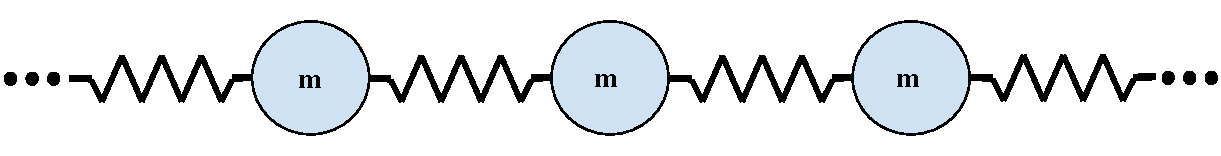
\includegraphics[width=0.75\textwidth]{mass-spring.pdf}
	\caption{A system of masses connected by springs extending infinitely to 
	the left and right.}
	\label{fig:ms}
\end{figure}
The equation of motion for the $n$th mass in the system is
\begin{equation} \label{eqnms}
m\frac{\partial^2 u_n}{\partial t^2} = k(u_{n-1} - u_n) - k(u_n - u_{n+1}) = 
ku_{n-1} - 2ku_n + ku_{n+1} 
\end{equation}
where $u_n$ gives the displacement of the $n$th node and $k$ is the spring 
constant of each spring. To acquire the dispersion relation for this system we 
assume a Bloch wave solution of the form
\begin{equation} \label{bloch}
u_n(x,t) = \tilde{u}(x_n)e^{i(kx_n - \omega t)}
\end{equation}
$\tilde{u}(x)$ is the amplitude of the wave and $x_n = nl$ where $l$ is the 
distance between the masses. Substituting the above into the equation of motion
\begin{align*}
-m \omega^2 u_n   &= ke^{i(k(n-1)l - \omega t)} - 2ku_n + ke^{i(k(n+1)l - 
\omega t)} \\
&= ke^{-ikl}u_n + ke^{ikl}u_n - 2ku_n \\
&= k\cos(kl)u_n - 2ku_n
\end{align*}
Thus,
\begin{equation}
\left[2\omega_0^2(1 - \cos(kl)) - \omega^2\right]u_n = 0
\end{equation}
where $\omega_0 = \sqrt{k/m}$ The above has a trivial solution when $u_n = 0$. 
Not so trivial solutions exist when
\begin{equation}
2\omega_0^2(1 - \cos(kl)) - \omega^2= 0
\end{equation}
We can write the dispersion relation for waves propagating through our mass 
spring system as
\begin{equation} \label{monatomicdisp}
\omega = \pm \sqrt{2\omega_0^2(1 - \cos(kl))}
\end{equation}
It is now becoming apparent that in a system of $n$ masses and springs that 
there is dispersion. To see this explicitly, write the phase velocity
\begin{equation}
v_p = \frac{w(k)}{k} = \frac{\pm\sqrt{2\omega_0^2(1 - \cos(kl))}}{k}
\end{equation}
Clearly, the phase velocity is a function of wave number/frequency which 
indicates dispersivity of the system.

Take our dispersion relation (\ref{monatomicdisp}) and nondimensionalize by 
letting $\Omega=\frac{\omega}{\omega_0}$ and $\mu=kl$. Then,
\begin{equation}
\Omega = \pm \sqrt{2(1-cos(\mu))}
\end{equation}
The positive part is plotted in Figure \ref{fig:dr}. Notice that it is periodic 
in $\mu$. The section of the dispersion relation from $-\pi$ to $\pi$ is called 
the first Brillouin zone. Due to symmetry, we also define the irreducible 
Brillouin zone (IBZ) as the section from $0$ to $\frac{\pi}{2}$. 
\begin{figure}[!htbp]
	\centering
	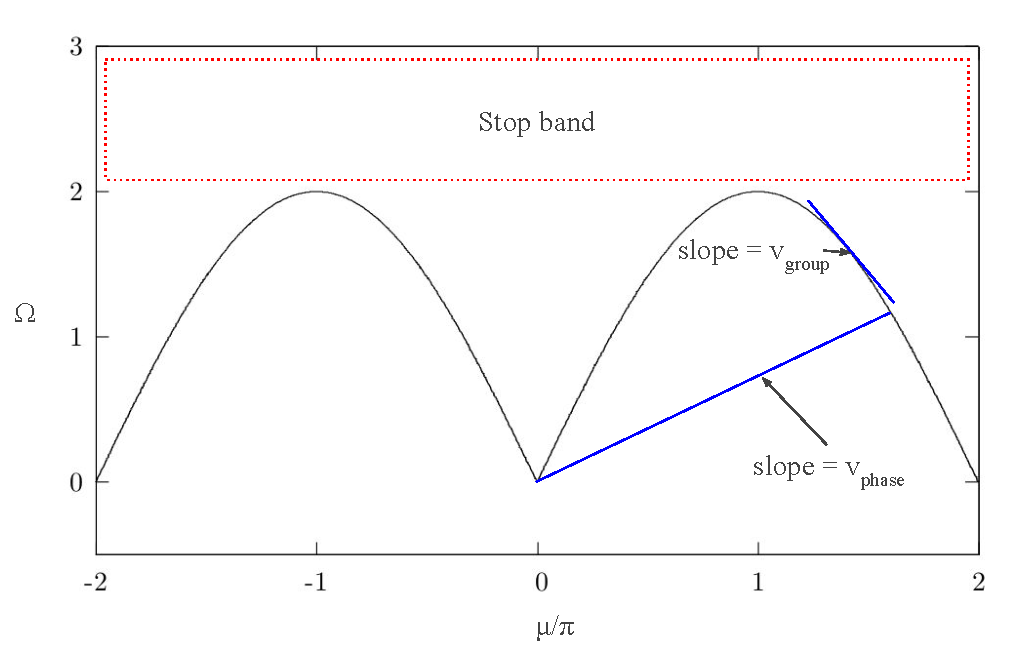
\includegraphics[width=0.6\textwidth]{dispersion-rln.pdf}
	\caption{The non-dimensional dispersion relation for the mass spring system}
	\label{fig:dr}
\end{figure}
The dispersion relation characterizes many features of the mass-spring system. 
In Figure \ref{fig:dr}, it is easy to identify the phase and group velocities 
along the curve for different waves propagating through the system. 

At first glance, it appears that there are no frequencies above $\Omega = 2$. 
In this region (called the stop band), waves experience attenuation and 
exponentially die off. Wave numbers in the stop band are imaginary. Looking at 
(\ref{bloch}), it becomes obvious where the attenuation comes from. Waves whose 
wave numbers are imaginary are called \emph{evanescent} waves.

Solving for wavenumber in terms of a given frequency 
\begin{equation} \label{imagwavenum}
\mu = \arccos{\left(1-\frac{\Omega^2}{2}\right)}
\end{equation}
We see that when $\Omega > 2$ the wave number becomes complex valued. The 
expression for (\ref{imagwavenum}) when we extend the values of $\mu$ into the 
complex plane is 
\begin{equation}
		\mu = -i\log \left[ \xi + i(1-\xi^2)^\frac{1}{2} \right]
\end{equation}
where
\begin{equation}
	\xi = 1-\frac{\Omega^2}{2}
\end{equation}
The implication here is that when the wave number becomes imaginary the $i$ in 
the wavenumber will multiply with $i$ in (\ref{bloch}) resulting in a 
exponential decay of the solution in space. This means there is no wave 
propagation.

\subsubsection{Diatomic lattice}
Next, we consider a diatomic lattice as shown in Figure \ref{fig:dms} with 
alternating masses, but springs of the same spring constants. There are two 
ways to solve this problem. The first is called the inverse method which 
imposes a wave number and gives frequencies. The second is the 
direct method which imposes a frequency and gives wave numbers. We will use the 
inverse method for the diatomic lattice and later for a laminate use the 
transfer matrix method.
\begin{figure}[!htbp]
	\centering
	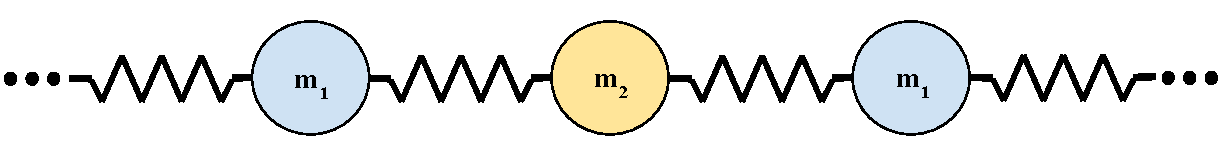
\includegraphics[width=0.75\textwidth]{diatomic-mass-spring.pdf}
	\caption{A system of alternating masses connected by springs extending 
	infinitely to the left and right.}
	\label{fig:dms}
\end{figure}
After assuming a harmonic motion
\begin{equation}
u_n = \tilde{u}(x_n)e^{i\omega t}
\end{equation}
The equations of motion for a diatomic lattice can be written
\begin{align}
	(-\omega^2m_2 + 2k)u_{2n} - k(u_{2n-1} + u_{2n+1}) &= 0 \\
	(-\omega^2m_1 + 2k)u_{2n+1} - k(u_{2n} + u_{2n+2}) &= 0
\end{align}
We can write this in a matrix form
\begin{equation}
(\mathbf{K}_n - \omega^2 \mathbf{M})\mathbf{u}_n + 
\mathbf{K}_{n-1}\mathbf{u}_{n-1}
+ \mathbf{K}_{n+1}\mathbf{u}_{n+1} = 0
\end{equation}
where
\begin{equation}
\mathbf{u}_n =
\begin{bmatrix}
u_{2n} \\
u_{2n+1}
\end{bmatrix}
\end{equation}
We will use the inverse method to solve for the dispersion relation. We use 
Bloch's theorem to write
\begin{equation}
\mathbf{u_n}= \mathbf{\hat{u}}(\mu)e^{in\mu}
\end{equation}
Finally, we can write
\begin{equation}
\left[\mathbf{K}_n + \mathbf{K}_{n-1}e^{-i\mu} + \mathbf{K}_{n+1}e^{i\mu} 
-\omega^2 \mathbf{M} \right] \mathbf{\hat{u}}(\mu)e^{in\mu} = 0
\end{equation}
and condensing all of the stiffness matrices
\begin{equation}
\left[\mathbf{\tilde{K}}(\mu) -\omega^2 \mathbf{M} \right] 
\mathbf{\hat{u}}(\mu)e^{in\mu} = 0
\end{equation}
Calculating the determinant of the matrix on the left we get the relation
\begin{equation}
\omega =\pm \sqrt{k\frac{m_1+m_2}{m_1m_2} \pm k 
\sqrt{\left(\frac{m_1+m_2}{m_1m_2}\right) - \frac{4(\sin{\mu})^2}{m_1m_2}}}
\end{equation}
The dispersion relation for the diatomic lattice is shown in Figure 
\ref{fig:dia-exact}. Notice that there are now two curves unlike in the 
monatomic case. Each curve corresponds to a mode of vibration where in this 
case the bottom one is called the acoustic mode and the top is called the 
optical mode. Another notable feature is the formation of a band gap in between 
the two modes. Like the monatomic case the wavenumbers become imaginary in this 
region. Additionally, there is still a stop band, but in this case the cutoff 
frequency is lower -about $\Omega = 1.75$.
\begin{figure}[!htbp]
	\centering
	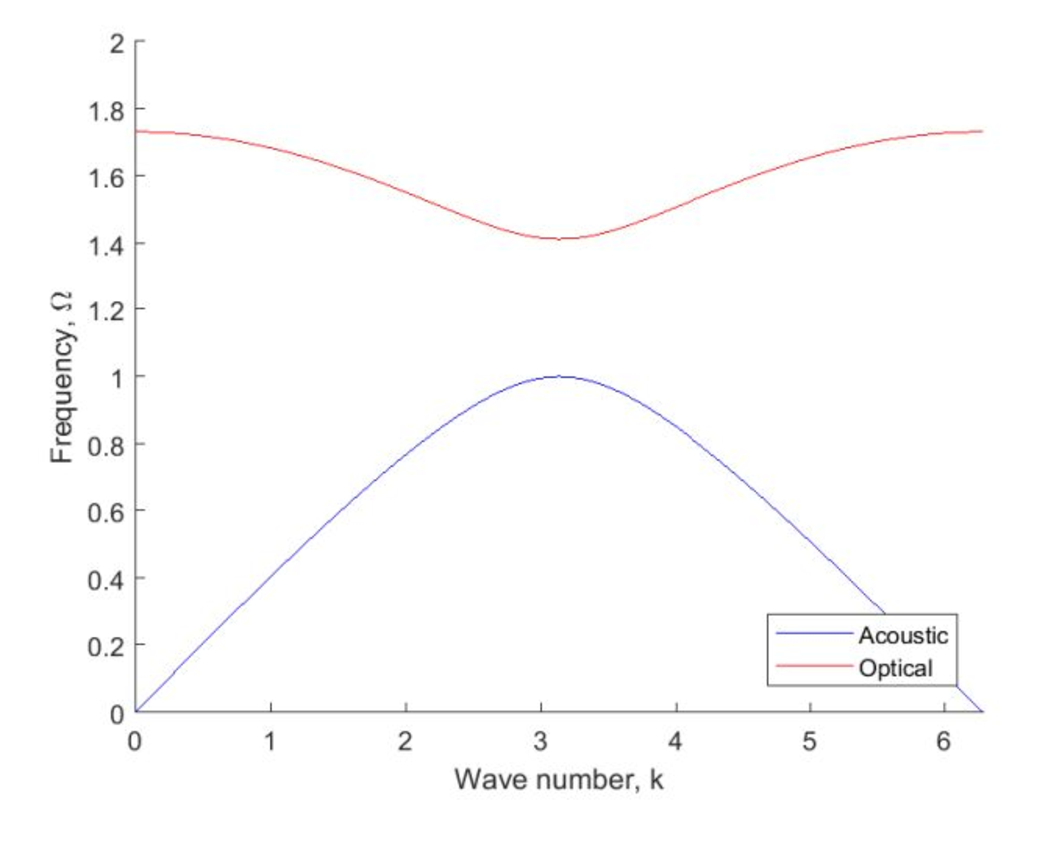
\includegraphics[width=0.6\textwidth]{diatomic-exact.pdf}
	\caption{Dispersion relation for the diatomic lattice system with 
	$m_1=1$, $m_2=2$, and $k=1$.}
	\label{fig:dia-exact}
\end{figure}

\subsubsection{Laminate}
The transfer matrix method enforces continuity between layers of a system. At 
the interface between two unit cells the displacements must be equal and the 
forces or tractions must be as well. First, a relationship between these 
variables must be derived from one end of the unit cell to the other end. The 
relationship can be written in a matrix called the  transfer matrix. This type 
of analysis is completed by applying Bloch's theorem to relate the 
displacements and forces in one cell to another. Here we outline the anlaysis 
of Shmuel \cite{shmuel16}

Consider a two phase laminate, with layer thicknesses $h^{(p)}$ and lamination 
direction $n$. A plane wave in layer $i$ that is propagating in the direction 
of $n$ has the general form
\begin{equation}
	u^{(p)} = m^{(p)}e^{ik^{(p)}(n\cdot x - c^{(p)} t)}
\end{equation}
where $m^{(p)}$ is the polarization and $c^{(p)}$ is the wave speed. From the 
above and the constitutive equations for linear elasticity, a relationship for 
the displacements at each end of a single layer can be written
\begin{equation} \label{transfeqn}
	\begin{bmatrix}
		u^{(p)}(x+h^{(p)}n,t) \\
		t^{(p)}(x+h^{(p)}n,t)
	\end{bmatrix}
	=
	\begin{bmatrix}
		\cos{ k^{(p)} h^{(p)} } && \frac{\sin{ k^{(p)} h^{(p)} 
		}}{\tilde{\mu}^{(p)}k^{(p)}} \\
		- \tilde{\mu}^{(p)}k^{(p)} \sin{ k^{(p)} h^{(p)} } &&
		\cos{ k^{(p)} h^{(p)}}
	\end{bmatrix}
	\begin{bmatrix}
		u^{(p)}(x,t) \\
		t^{(p)}(x,t)
	\end{bmatrix}
\end{equation}
$\tilde{\mu}$ is a combination of Lam\'e constants which is different for 
transverse and longitudinal waves. The matrix $T^{(p)}$ is the transfer matrix 
for one layer.

In order to relate, the displacements at the opposite ends of the unit cell of 
this two phase laminate we need two transfer matrices.
\begin{equation} \label{transfeqn}
	\begin{bmatrix}
		u^{(1)}(x+h^{(1)}n+h^{(2)}n,t) \\
		t^{(1)}(x+h^{(1)}n+h^{(2)}n,t)
	\end{bmatrix}
	=
	T^{(2)}T^{(1)}
	\begin{bmatrix}
		u^{(1)}(x,t) \\
		t^{(1)}(x,t)
	\end{bmatrix}
\end{equation}
At this point, we use Bloch's theorem to enforce that the displacements at the 
boundary of the unit cell must be equal up to a phase constant. The end result 
is an equation of the form
\begin{equation}
	\left(T^{(2)}T^{(1)} - \lambda I\right)
	\begin{bmatrix}
		u^{(1)}(x,t) \\
		t^{(1)}(x,t)
	\end{bmatrix} = 0
\end{equation}
where $\lambda = e^{ik_bh}$ (h is the width of the unit cell) and $k_b$ is the 
Bloch wavenumber. The determinant of the matrix must be equal to zero which 
generates a dispersion relation. Given a frequency $\omega$ , the dispersion 
relation gives a set of corresponding $k_b$ (where
$\omega=c^{(p)}k^{(p)}$ in the above equations).

%----------------- COMPUTATIONAL METHODS FOR PHONONIC MEDIA -------------------%
%  We jut got done talking a lot about dispersion relations. To make this jump
%  Computational methods we need make a point about how for nontrivial systems
%  and continuum systems that sort of analysis isn't as realistic
%  also talk about why we are specializing in finite elements. When you get to
%  finite elements explain what is actually happening in the code for people
%  who aren't as familiar with these computational methods
%------------------------------------------------------------------------------%
\section{Computational methods for phononic media} \label{methods}
While we were able to derive explicit dispersion relations in the examples 
given in the previous section, it is quickly becomes unfeasible even for some 
2D and most 3D cases. We must turn to computational analysis in these cases in 
order to compute the dispersion relations for these phononic media. Here the 
four most prominent methods in the literature are the plane-wave expansion 
method, finite difference method, finite element method, and the multiple 
scattering method. Each is explained briefly in this section, however, for the 
independent study we choose to specialize in the finite element method which 
will also be used in further research.

According to \cite{cao04}, the plane-wave method is widely used because of its 
convenience. Apparently, the drawback of this method is slow convergence. In 
general, the displacements and material properties are first expanded in a 
series related to the lattice vectors and a Bloch wave solution is asserted. 
These expansion are substituted back into the wave equation which after some 
manipulation leads to an eigenvalue problem \cite{hussein14}.

Finite difference methods are similar to the plane wave expansion method with 
the advantage that the solution convergence is faster for materials with 
multiple phases. Instead of expanding the solution and material properties, the 
differential operators of the wave equation are approximated using standard 
finite difference formulas. At this point, it is possible to solve the 
equations at various time steps to obtain the real time evolution of the 
system. From the real time evolution, it is possible to take the Fourier 
transform of the data in order to obtain the wave number of a wave for which 
the excitation frequency is known and thus form a dispersion relation. 
Alternatively, asserting a Bloch wave solution after using the finite 
difference approximation results in an eigenvalue value problem that yields 
eigenfrequencies given an imposed wave number. 

The finite element method is useful for complex material geometries. A weak 
from of the governing equations is still 
formulated by multiplying by a trial function, but the integration is performed 
only over a unit cell which represents the phononic medium of interest. After 
approximating the solution and trial function with appropriate weight 
functions, we can proceed in two ways much like in the finite difference 
method. It is possible to use a central difference approximation for the time 
derivative and calculate the real time evolution (for more detail see Appendix 
\ref{femrte}). This, however, is 
computationally inefficient. Instead, we apply Bloch's theorem. In this case, 
Bloch's theorem can be used to impose a Bloch condition on the 
boundary which reduces the degrees of freedoms of the system by relating the 
displacements at one boundary to the opposite boundary plus a phase multiplier.
This process results in an eigenvalue problem similar to the above two cases. 
As this method will be used in future studies, it will be elaborated on in 
detail in upcoming sections.

Compared to the above methods, the multiple scattering method has an advantage 
when the material under consideration contains scattering elements. The method 
relies on separating the solution into fields associated with the incident wave 
and then waves scattered from each scattering element in the system. Once the 
solution, at a single scattering element a system of equations can be solved 
for the rest of the scattered fields. The dispersion relations are then found 
by application of Bloch's theorem. 

%---------- ANALYSIS OF LATTICE STRUCTURES VIA REAL TIME EVOLUTION ------------%
%  Real time evolution is sort of like a finite difference method right? But it 
%  is not the finite difference scheme described above. You are going to have 
%  frame this correctly so that the audience knows why this type of analysis 
%  is useful. Really, how does looking at the real time evolution fit the 
%  story you are trying to tell about dispersion relations and and this whole 
%  thing with Bloch's theorem
%------------------------------------------------------------------------------%
\section{Analysis of lattice structures via real time evolution}
Here, the monatomic and diatomic lattice systems are computationally realized
using the finite difference time domain method. A Bloch wave solution is not 
imposed which will allow us to directly visualize the behavior of the 
system inside and outside of the band gaps and stop bands. Additionally, the 
(discrete) Fourier transform of the real time evolution data is taken in order 
to find the dispersion relations in each case. 

\subsection{Monatomic lattice}
A monatomic lattice with 100 masses is modeled using the equations of motion 
(\ref{eqnms}) and the Verlet integration method. The Verlet integration method 
is involves a central difference approximation for the time derivative in 
Newton's equations. See Appendix \ref{verlet} for more details on the Verlet 
integration method. One end of the system is subject to a harmonic excitation 
with a prescribed frequency, and the other end is allowed to freely move. For 
the material parameters, we choose $m=1$ and $k=1$.

In order to compute the dispersion relation of the system, a range of 
frequencies is prescribed from $\Omega=0$ to $\Omega=2$. At each frequency and 
after allowing the system to evolve in time, a Fourier transform of the system 
is taken in the space domain. From the Fourier transform of the displacements, 
which is now in the wavenumber domain (recall that the wave number can be 
thought of as the spatial frequency of the wave), the location of the peak of 
the spectrum is taken as the wavenumber for the corresponding excitation 
frequency. The result is Figure \ref{fig:matlab-dr}.
\begin{figure}[!htbp]
	\centering
	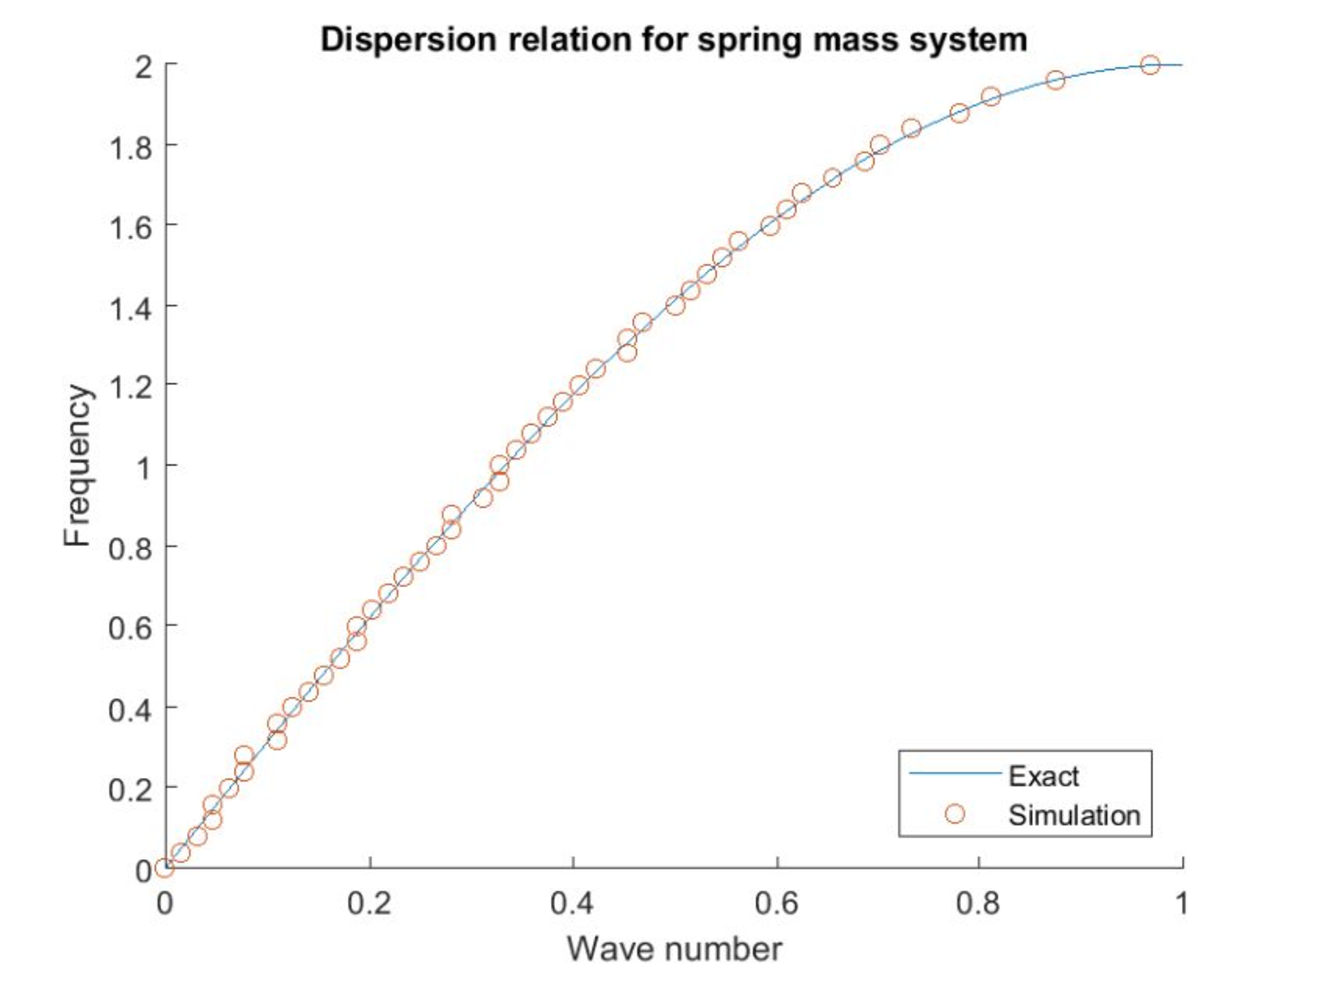
\includegraphics[width=0.6\textwidth]{matlab-dr.pdf}
	\caption{Using a Fourier transform in space, wave lengths for different 
	excitation frequencies are identified and plotted}
	\label{fig:matlab-dr}
\end{figure}
The results are in good agreement with the derived dispersion relation, but 
there is noticeable error due to reflections at the free end of the chain. If 
the chain of masses was longer, this would not be less of a problem. 

Increasing the frequency of the harmonic excitation above the cutoff frequency 
of the system it is easy to explore the attenuation effect at the stop band as 
seen in Figure \ref{fig:dr}. Figures \ref{fig:snap19} and \ref{fig:snap21} 
display snapshots of the system at excitation frequencies above and below 
$\Omega=2$. There is an obvious drop in amplitude inside and outside of the 
stop band.
\begin{figure}[!htbp]
	\centering
	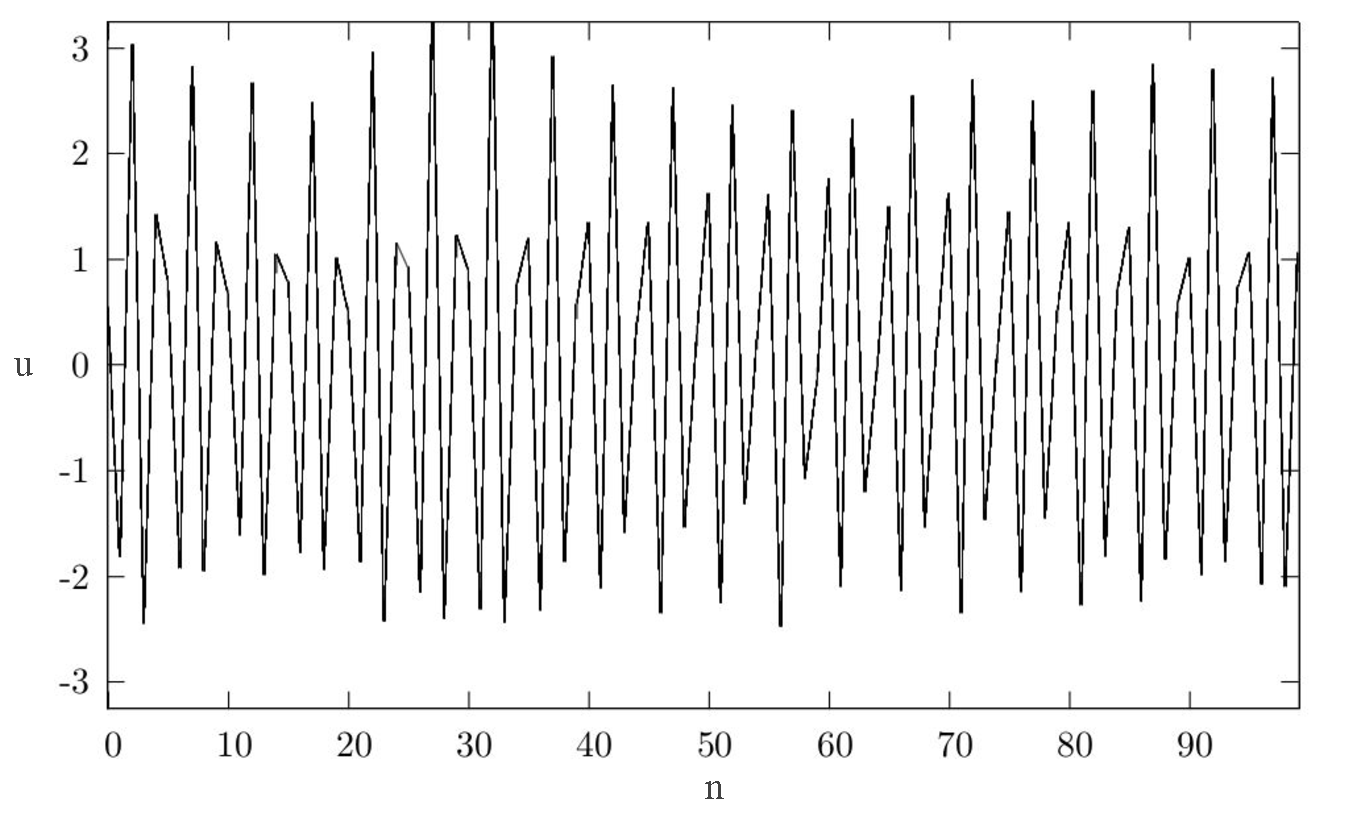
\includegraphics[width=0.6\textwidth]{snap-f19.pdf}
	\caption{Snapshot of mass spring system with $\Omega=1.9$}
	\label{fig:snap19}
\end{figure}
\begin{figure}[!htbp]
	\centering
	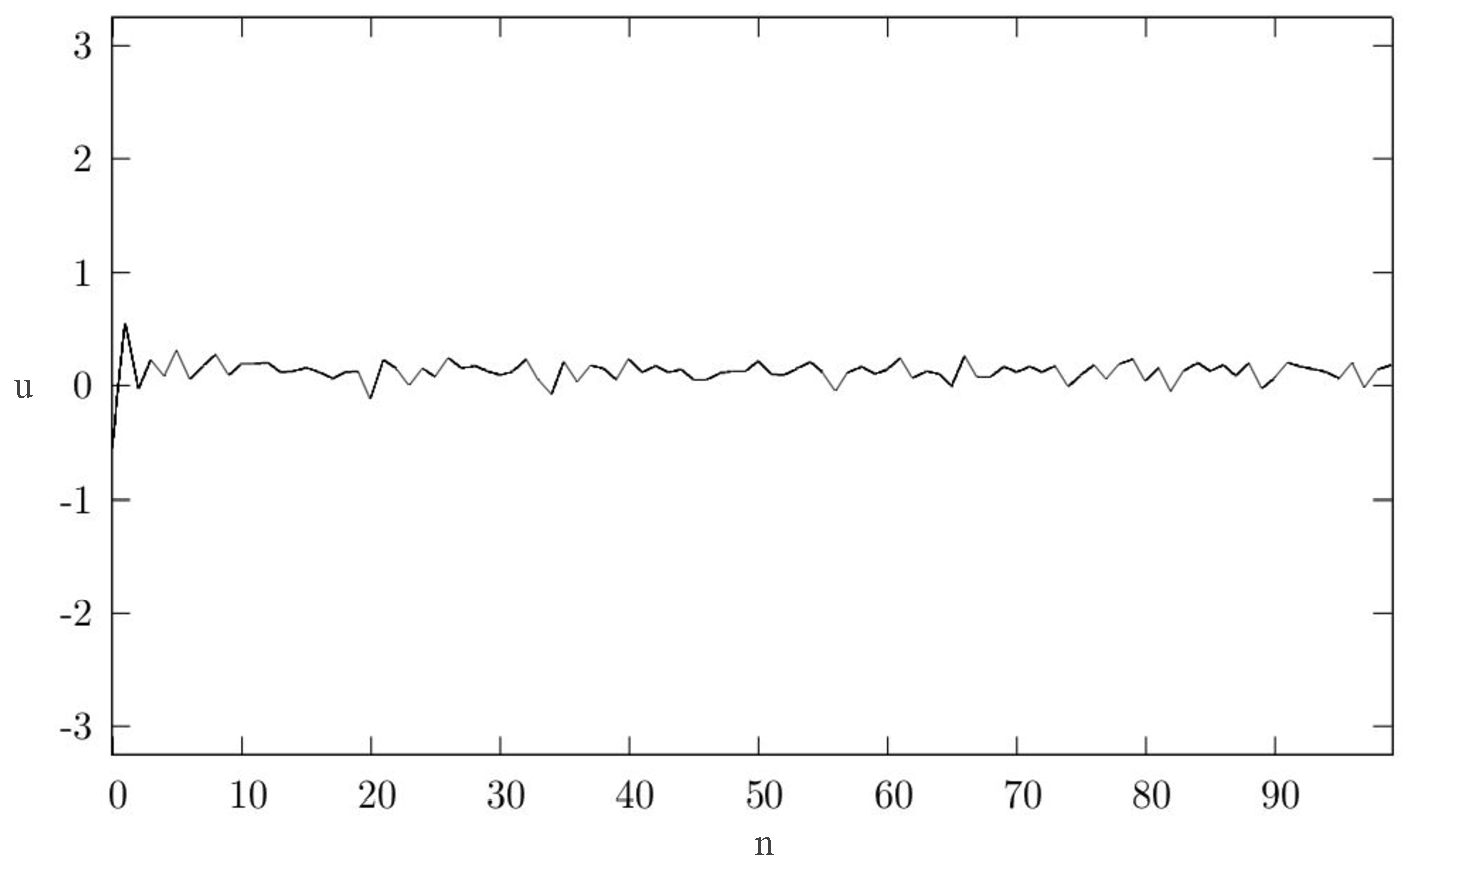
\includegraphics[width=0.6\textwidth]{snap-f21.pdf}
	\caption{Snapshot of mass spring system with $\Omega=2.1$}
	\label{fig:snap21}
\end{figure}

From the finite difference time domain method, it is also possible to calculate 
the values of the imaginary wavenumbers that occur for frequencies above cutoff 
frequencies. This is done by fitting a complex exponential to the evanescent 
waves and finding the power of the exponential term. Figure 
\ref{fig:imagwavenumres} has the results of 
the fitting process overlaid on top of the exact plot of the evanescent 
wavenumbers. 
\begin{figure}[!htbp]
	\centering
	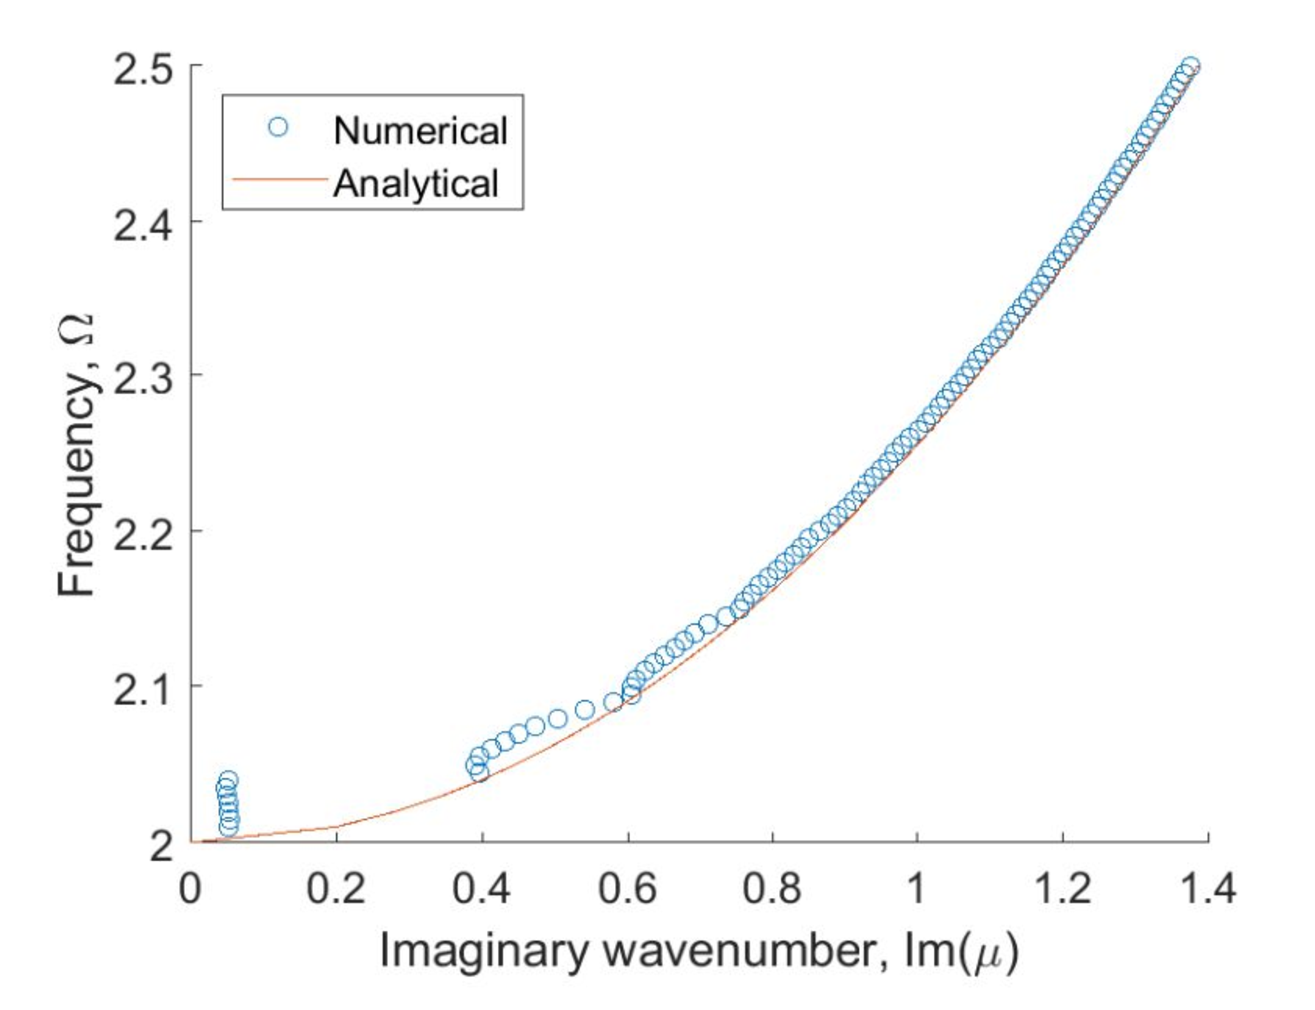
\includegraphics[width=0.6\textwidth]{im-wavenum-res.pdf}
	\caption{Here, the results of the exponential fitting process of the 
	evanescent waves are plotted.}
	\label{fig:imagwavenumres}
\end{figure}
Closer to the cutoff frequency, the results are not in good agreement. This is 
due to the reflections of the wave at the boundary of the system. 

Another way to identify band gaps in a system without calculating the Fourier 
transform is by comparing the amplitude of harmonic excitation to 
the maximum displacement at the free end. Sweeping over frequencies and 
plotting the 
ratio of displacements at each end results in a transmission loss diagram as in 
Figure \ref{fig:tlms}.
\begin{figure}[!htbp]
	\centering
	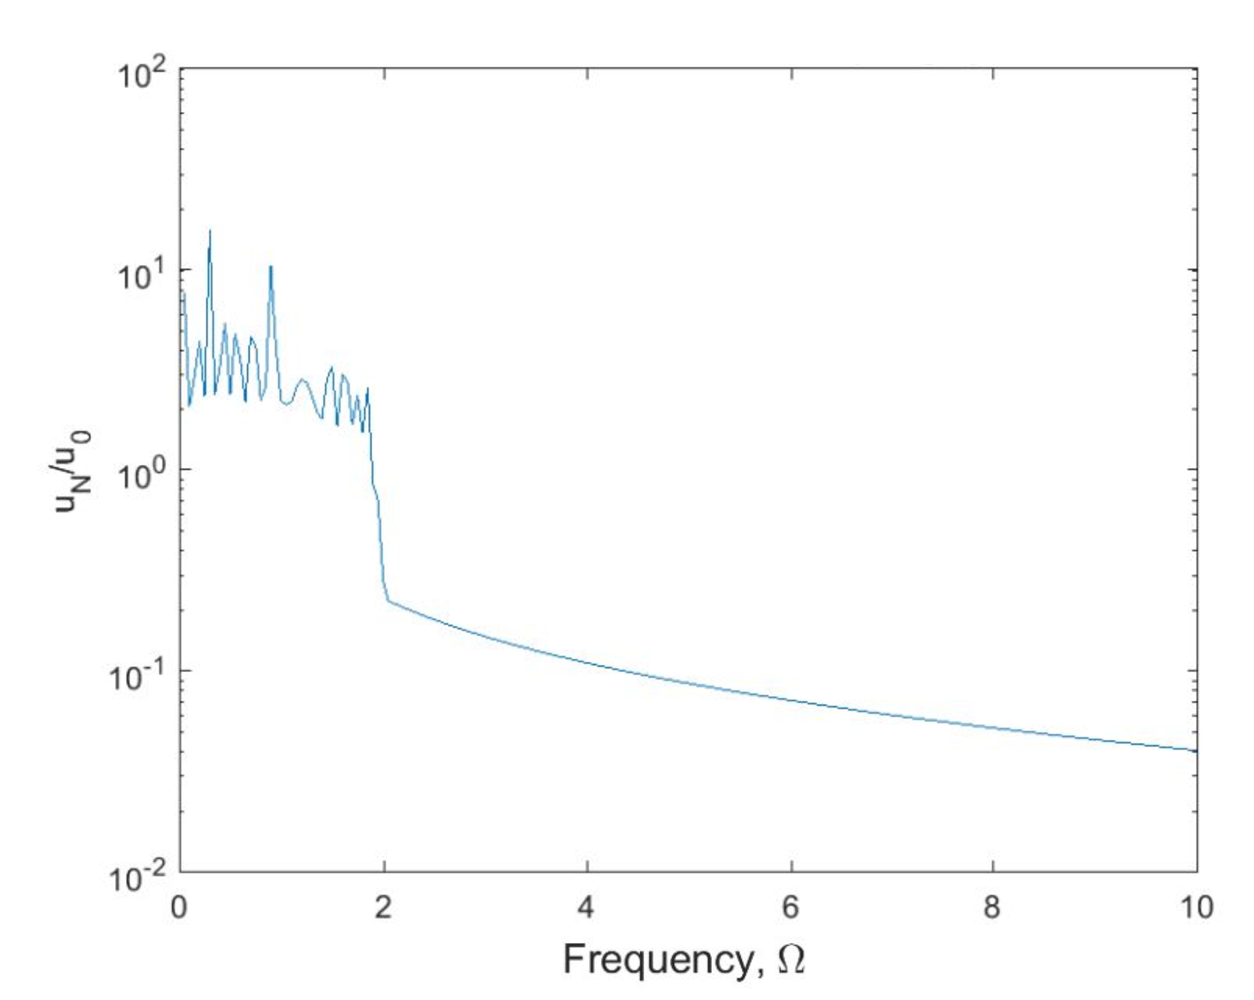
\includegraphics[width=0.6\textwidth]{tl-diag.pdf}
	\caption{The displacement of the excited mass and the free mass are 
	compared to construct this transmission-loss diagram.}
	\label{fig:tlms}
\end{figure}
It is apparent from Figure \ref{fig:tlms} that there is a cutoff frequency at 
$\Omega=2$. This may be inferred even before seeing the dispersion relation of 
the monatomic lattice beforehand.

\subsection{Diatomic lattice}
We also perform a finite difference time domain analysis for the diatomic 
lattice with $m_1=1$, $m_2=2$, and $k=1$. The results from taken the Fourier 
transform of the data and also the previously derived analytical expressions 
are plotted in Figure \ref{fig:diadr}.
\begin{figure}[!htbp]
	\centering
	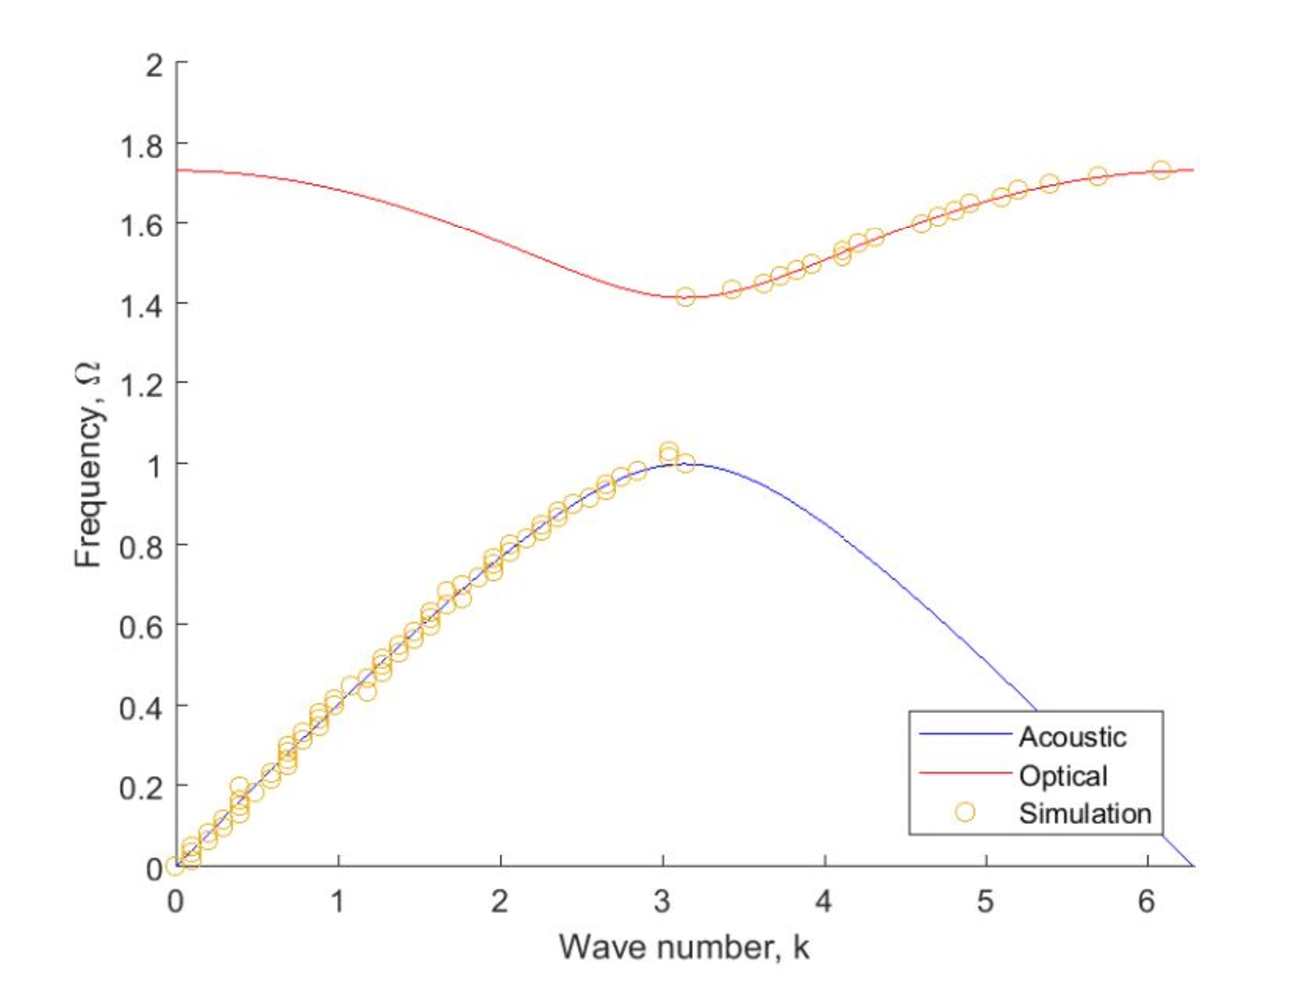
\includegraphics[width=0.6\textwidth]{diatomic-dr.pdf}
	\caption{The results for the finite difference time domain method are 
	plotted along side the exact dispersion relation derived using the inverse 
	method.}
	\label{fig:diadr}
\end{figure}
From the real time evolution we are able to recover the band gap between the 
two modes of vibration and also the stop band. Additionally, the 
transmission-loss diagram is also plotted in Figure \ref{fig:tlds} to 
illustrate the attenuation that the system undergoes.
\begin{figure}[!htbp]
	\centering
	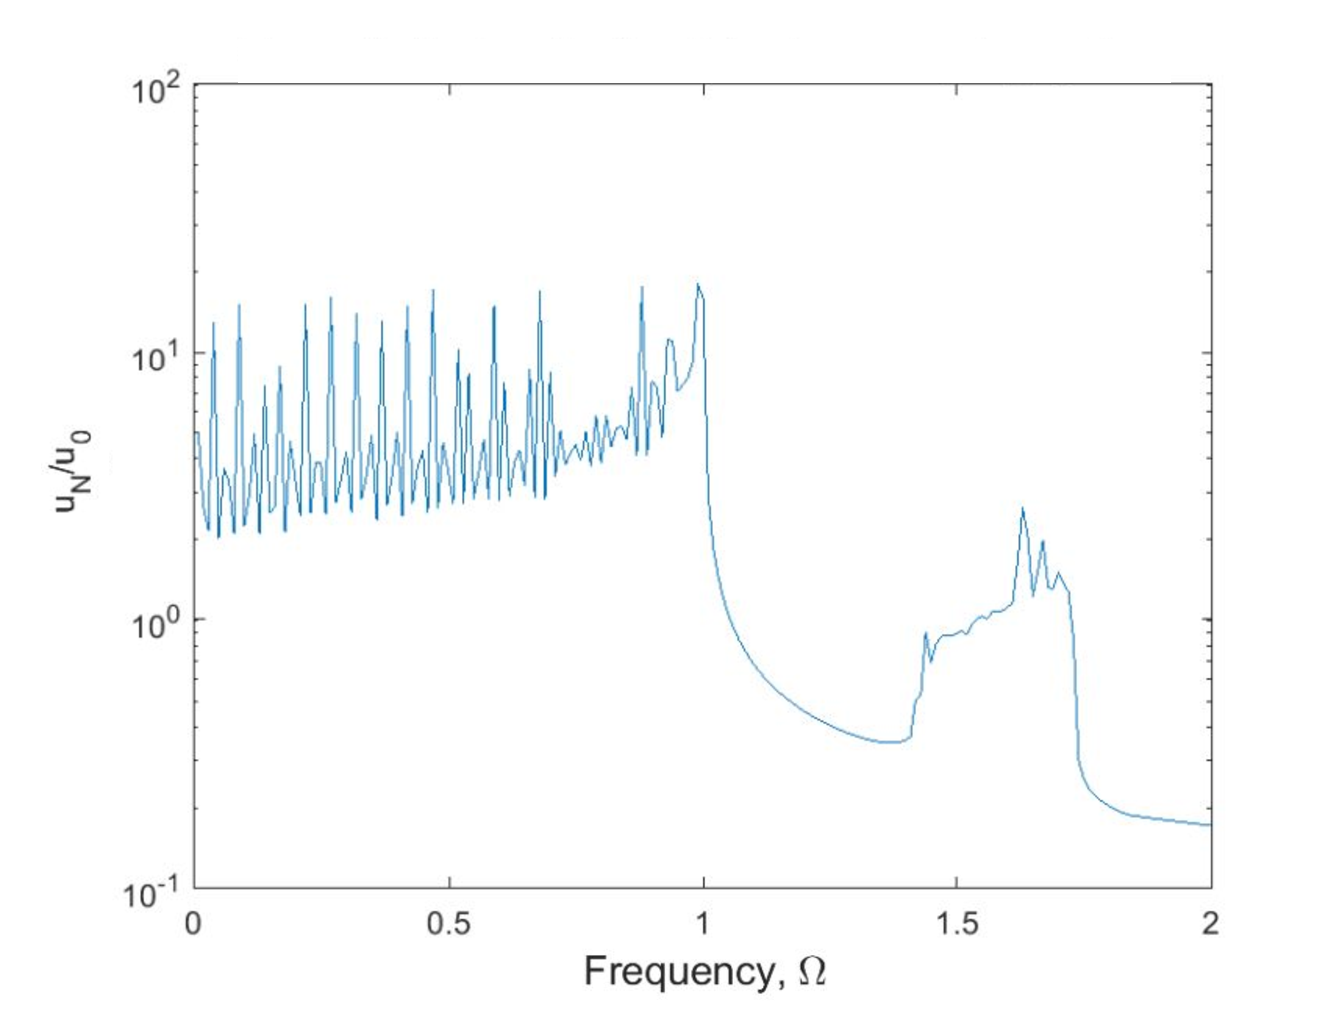
\includegraphics[width=0.6\textwidth]{dia-tl-diag.pdf}
	\caption{The displacement of the excited mass and the free mass in the 
	diatomic lattice are compared to construct this transmission-loss diagram.}
	\label{fig:tlds}
\end{figure}
It does appear that there is attenuation in the band gap and above the stop 
band. 

%------ ANALYSIS OF 1D CONTINUUM MATERIALS VIA FINITE ELEMENT METHOD ----------%
%  Here is where you connect with Bloch's theorem and what is a powerful method 
%  of analysis that will be used in actual research. Emphasize the importance 
%%%  of this and its utility.
%------------------------------------------------------------------------------%
\section{Analysis of 1D continuum materials via finite element method}
\subsection{Uniform bar}
As a first exercise in using finite elements to find the dispersion properties 
of materials, we will consider a uniform bar in one dimension. For the one 
dimensional problem, the elasticity equations we want to solve are.
\begin{align}
\frac{\partial \sigma_x}{\partial x} + b_i &= \rho \frac{\partial^2 
u_x}{\partial t^2},\quad x\in[0,L]\quad\textnormal{(Equilibrium)} \\
\sigma_x &= E \varepsilon_x\quad\textnormal{(Constitutive relation)}\\
\varepsilon_x &= \frac{\partial u_x}{\partial 
x}\quad\textnormal{(Strain-displacement)}\\
u_x(x=0,t) &= A_0sin(\omega t) \\
\sigma_x(x=L,t) &= 0
\end{align}

In the absence of body forces, we can find the weak form of the equilibrium 
equation by multiplying by a test function $\varphi$ and integrating of the 
domain.
\begin{equation}
\int_0^L \varphi \frac{\partial \sigma_x}{\partial x} dx
= \int_0^L \varphi \rho \frac{\partial^2 u_x}{\partial t^2} dx
\end{equation}
Using integration by parts on the LHS of the above we find that
\begin{equation}
\varphi(L)\sigma_x(L) - \varphi(0)\sigma_x(0) 
- \int_0^1 \frac{\partial \varphi}{\partial x} \sigma_x dx
= \int_0^L \varphi \rho \frac{\partial^2 u_x}{\partial t^2} dx
\end{equation}
Applying boundary conditions, constitutive relation, and the 
strain-displacement equation we arrive at the weak form of the equation
\begin{equation}
\int_0^1 \frac{\partial \varphi}{\partial x} E \frac{\partial u_x}{\partial x} 
dx
+ \int_0^L \varphi \rho \frac{\partial^2 u_x}{\partial t^2} dx = 0
\end{equation}
Now, we approximate our test function and solution using linear shape functions
\begin{align}
\varphi &= N_i(x) \\
u_x &= \sum_j a_j(t)N_j(x)
\end{align}
Then,
\begin{equation}
\int_0^1 \frac{\partial N_i(x)}{\partial x} E \sum_j\frac{\partial 
N_j(x)}{\partial x} a_j dx
+ \int_0^L N_i \rho \sum_j N_j \frac{\partial^2 a_j(t)}{\partial t^2} dx = 0
\end{equation}
Rearranging,
\begin{equation}
\int_0^1  E \sum_j\frac{\partial N_i(x)}{\partial x}\frac{\partial 
N_j(x)}{\partial x} a_j dx
+ \int_0^L \rho \sum_j  N_i N_j \frac{\partial^2 a_j(t)}{\partial t^2} dx = 0
\end{equation}
Finally, we write the above equation in matrix form
\begin{equation} \label{matrixform}
Ka+M\ddot{a} = 0 
\end{equation}
where $K$ is called the stiffness matrix, and $M$ is called the mass matrix. 

We now assume a harmonic solution of the form
\begin{equation}
a = \tilde{a}e^{i \omega t}
\end{equation}
such that the second order differential equation (\ref{matrixform}) becomes a 
complex eigenvalue problem:
\begin{equation}
Ka - \omega^2 Ma = (K-\omega^2M)a = 0
\end{equation}
Note that as of now $K$ and $M$ are not functions of the wave number and 
solving the eigenvalue problem as is does not yield any information about the 
dispersion properties of the system. To obtain this dependence the Bloch 
condition must be enforced. 

The Bloch condition is similar to the periodic boundary condition and is a 
manifestation of Bloch's theorem much like the Bloch wave solution that was 
asserted when analytically solving for the dispersion relation
\begin{equation}
a(x+h) = a(x)\quad\textnormal{(Periodic boundary condition)}
\end{equation}
where h is the size of the unit cell. The difference between the two conditions 
is a single multiplicative factor:
\begin{equation}
a(x+h) = e^{ik_xh}a(x)\quad\textnormal{(Bloch condition)}
\end{equation}
The multiplicative factor in the boundary condition shifts is such that when 
the wave reaches a boundary it is phase shifted to match the wave at the 
opposite boundary such that there is no interference.

Enforcing the condition is done via a linear transformation which in one 
dimension is
\begin{equation}
T = 
\begin{bmatrix}
1 && \mathbf{0} \\
\mathbf{0} && \mathbf{I}\\
e^{ik_xh} && \mathbf{0}
\end{bmatrix}
\end{equation}
where $\mathbf{I}$ is an identity matrix with dimensions equal to the number of 
interior nodes (in the one dimensional case this is the total number of nodes 
minus two). Using this transformation matrix we reduce the number of degrees of 
freedoms in our system and write
\begin{equation}
a =
\begin{bmatrix}
a_{left} \\
a_{int} \\
a_{right}
\end{bmatrix}
= 
\begin{bmatrix}
1 && \mathbf{0} \\
\mathbf{0} && \mathbf{I}\\
e^{ik_xh} && \mathbf{0}
\end{bmatrix}
\begin{bmatrix}
a_{left} \\
a_{int}
\end{bmatrix}
= T \hat{a}
\end{equation}
Our eigenvalue problem is now
\begin{equation}
(K-\omega^2M)T\hat{a} = 0
\end{equation}
To make it so our matrix is square, and therefore invertible, we premultiply 
the equation by $\bar{T}^T$
\begin{equation} \label{evalprob}
(\hat{K} - \omega^2 \hat{M})\hat{a} = 0
\end{equation}
where
\begin{equation}
\hat{K}(k_x) = \bar{T}^T K T
\end{equation}
and 
\begin{equation}
\hat{M}(k_x) = \bar{T}^T M T
\end{equation}
We are now in position to extract the dispersion properties of the uniform bar. 
The eigenvalue problem is solved several times for values of $k_x$, and we 
obtain several corresponding values for $\omega$. The dispersion relation for 
the uniform bar is plotted in Figure \ref{fig:unifbar}.
\begin{figure}[!htbp]
	\centering
	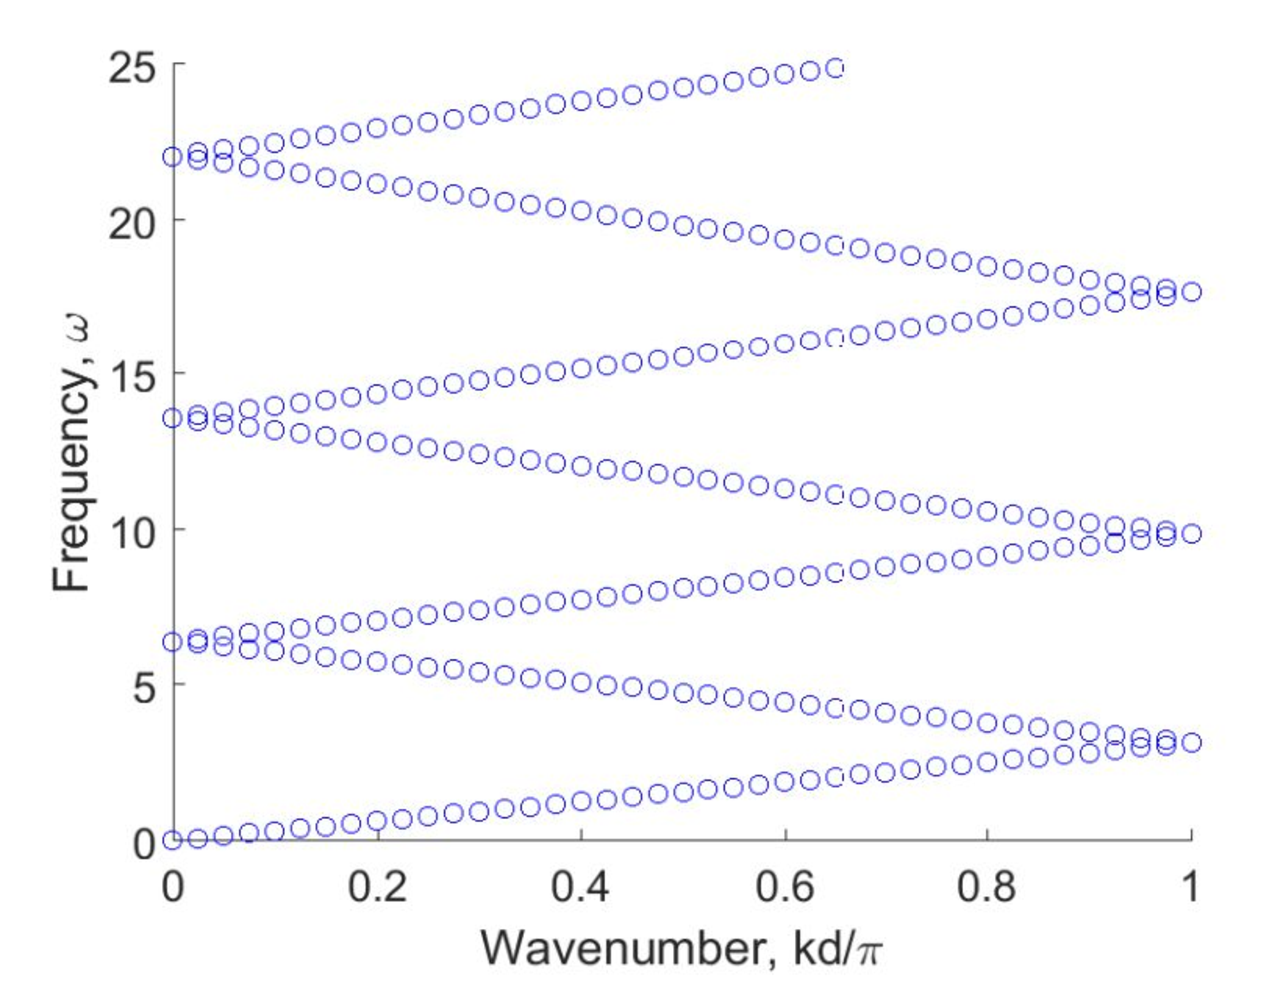
\includegraphics[width=0.6\textwidth]{unifbar.pdf}
	\caption{Dispersion relation for a uniform bar with $E=1$ and $\rho=1$.}
	\label{fig:unifbar}
\end{figure}
The dispersion relation has only has straight lines indicating there is no 
dispersion which is what we expect for a uniform material. No band gaps form 
because there are no periodic inclusions or structure to produce Bragg 
scattering. There are several modes corresponding to forward and backward 
propagating waves and it is verified that the wave speed is equal to one since 
when $k=\pm \omega$ for all wavenumbers.

\subsection{Layered composite}
For the layered composite, a bimaterial unit cell is consider as shown in 
Figure \ref{fig:layrdcell} with a stiffer and denser material in the center 
with length equal to that of a half the length of the unit cell. 
\begin{figure}[!htbp]
	\centering
	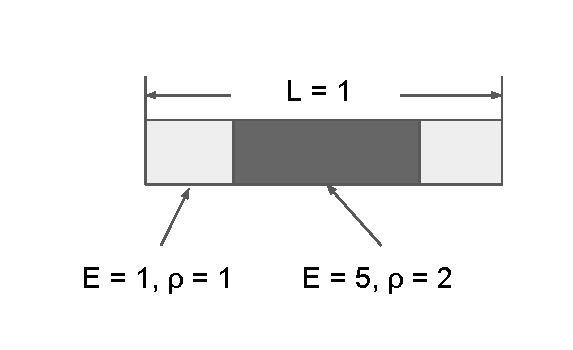
\includegraphics[width=0.5\textwidth]{layrd-unit-cell.pdf}
	\caption{Unit cell of the layered composite with each phase occupying an 
	equal volume fraction.}
	\label{fig:layrdcell}
\end{figure}
The same finite element analysis as performed on this layered composite 
resulting in the dispersion relation shown in Figure \ref{fig:layrd}.
\begin{figure}[!htbp]
	\centering
	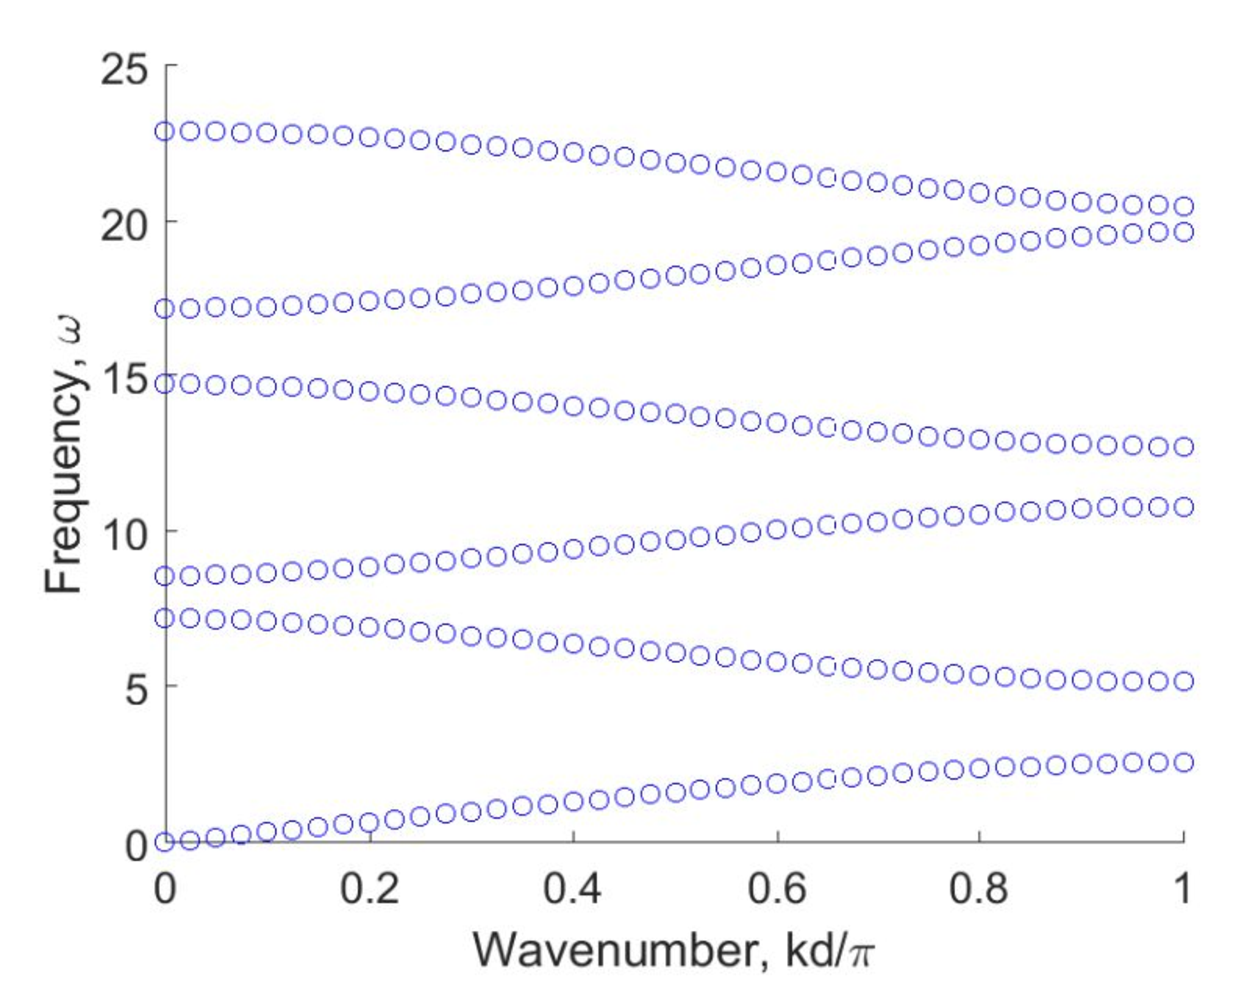
\includegraphics[width=0.6\textwidth]{layrd.pdf}
	\caption{Dispersion relation from the finite element analysis of a unit 
	cell of the layered composite}
	\label{fig:layrd}
\end{figure}
Due to the periodicity of the material, we see the formation of band gaps and 
the presence of dispersion. 

%------ ANALYSIS OF 2D CONTINUUM MATERIALS VIA FINITE ELEMENT METHOD ----------%
%  At this point you have already explained what finite elements is in 1D. You
%  will need to reiterate the process but explain in detail the new equations 
%  for 2D finite elements. Additionally, what new sorts of phenomena do we 
%  expect to see here. What are the difficulties? What are the new
%  consideration? What are the new results? etc.
%------------------------------------------------------------------------------%
\section{Analysis of 2D continuum materials via finite element method}
Extending finite elements to 2D, we find that after considering the principle 
of virtual work and approximating our solution using linear shape functions 
that 
\begin{equation}
\left[\int_{\Omega} (BN)^T C BN dV\right]a 
- \left[ \int_{\Omega} N^T \rho N dV \right]\ddot{a} = 0
\end{equation}
where
\begin{equation}
	N = 	
	\begin{bmatrix}
	N_1 & 0 & N_2 & 0 & ... & N_n & 0 \\
	0 & N_1 & 0 & N_2 & ... & 0 & N_n
	\end{bmatrix}
\end{equation}
and 
\begin{equation}
	B =
	\begin{bmatrix}
		\frac{\partial }{\partial x} & 0 \\
		0 & \frac{\partial }{\partial y} \\
		\frac{\partial }{\partial y} & \frac{\partial }{\partial x}
	\end{bmatrix}
\end{equation}
For our constitutive relation we consider an isotropic material with
\begin{equation}
	\sigma_{ij} = 2\mu\varepsilon_{ij} + \lambda\varepsilon_{kk}\delta_{ij}
\end{equation}
such that
\begin{equation}
	C = 
	\begin{bmatrix}
	2\mu+\lambda & \lambda & 0 \\
	\lambda & 2\mu + \lambda & 0 \\
	0 & 0 & 2\mu 
	\end{bmatrix}
\end{equation}
Note that this corresponds to a 2D material and not a 3D material in plane 
strain or plane stress.

We can write our matrix form in the same form as in the 1D case and also assume 
a harmonic solution.
\begin{equation} \label{twodfem}
Ka - M\ddot{a} = \left(K - \omega^2 M\right)a = 0
\end{equation}
Furthermore, we will apply the Bloch condition again. The linear transformation 
matrix is more complicated due to the added dimension. In order to impose the 
Bloch condition in 2D, the degrees of freedom of the unit cell must be divided 
into interior nodes and boundary nodes according to Figure 
\ref{fig:twodunitcell}.
\begin{figure}[!htbp]
	\centering
	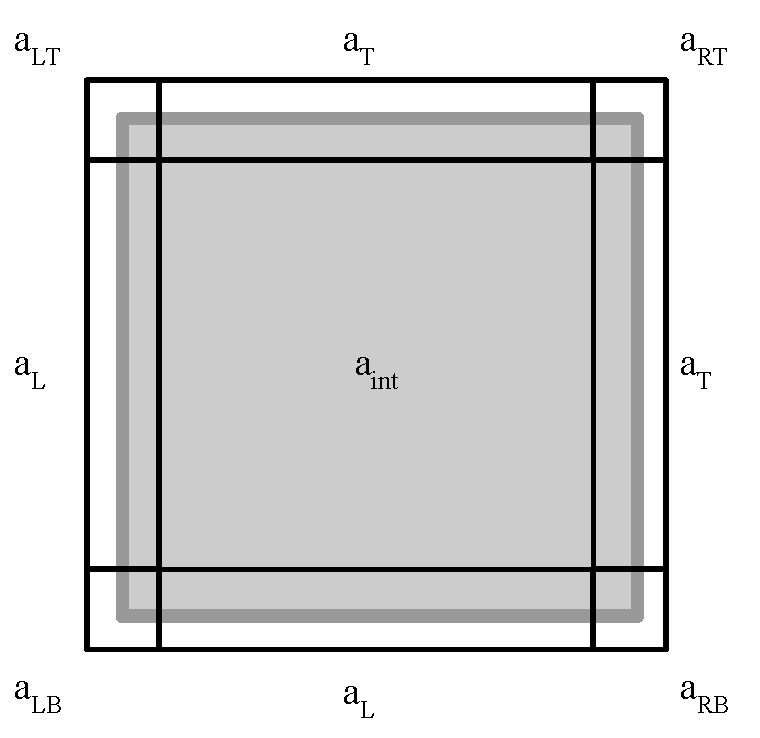
\includegraphics[width=0.55\textwidth]{twodunitcell.pdf}
	\caption{The degrees of freedom are partitioned into nodes at the left-top 
	(LT), right-top (RT), left-bottom (LB), right-bottom (RB) corners. 
	Non-corner nodes are further divided into right (R), left (L), top (T), 
	bottom (B) sides and also interior (int)}
	\label{fig:twodunitcell}
\end{figure}
Based on the aforementioned partitioning scheme, the degrees of freedom are 
reduced according to the following
\begin{equation}
a =
\begin{bmatrix}
a_{B} \\
a_{L} \\
a_{LB} \\
a_{int} \\
a_{T} \\
a_{R} \\
a_{RB} \\
a_{LT} \\
a_{RT} 
\end{bmatrix}
= 
\begin{bmatrix}
\mathbf{I} && \mathbf{0} && \mathbf{0} && \mathbf{0}\\
\mathbf{0} && \mathbf{I} && \mathbf{0} && \mathbf{0}\\
\mathbf{0} && \mathbf{0} && \mathbf{I} && \mathbf{0}\\ 
\mathbf{0} && \mathbf{0} && \mathbf{0} && \mathbf{I}\\
e^{ik_yh_y} && \mathbf{0} && \mathbf{0} && \mathbf{0} \\
\mathbf{0} && e^{ik_xh_x} && \mathbf{0} && \mathbf{0}\\
\mathbf{0} && \mathbf{0} && e^{ik_xh_x} && \mathbf{0}\\
\mathbf{0} && \mathbf{0} && e^{ik_yh_y} && \mathbf{0}\\
\mathbf{0} && \mathbf{0} && e^{ik_xh_x}e^{ik_yh_y} && \mathbf{0}\\
\end{bmatrix}
\begin{bmatrix}
a_{B} \\
a_{L} \\
a_{LB} \\
a_{int} 
\end{bmatrix}
= T \hat{a}
\end{equation}
Now we post- and pre- multiply \ref{twodfem} by $T$ and its complex conjugate 
$\bar{T}$ and obtain a complex eigenvalue problem similar to the 1D case. We 
then follow the same process of prescribing wavenumbers and solving the 
eigenvalue problem to obtain the corresponding frequencies.

\subsection{Uniform material}
Here we consider a uniform material with Lam\'e constants $\lambda=1$ and 
$\mu=1$. In order to fully characterize the wave propagation features of the 2D 
material, we only need to solve the eigenvalue equation for wave vectors in the 
irreducible Brillouin zone (IBZ) depicted in Figure \ref{bloch}.
\begin{figure}[!htbp]
	\centering
	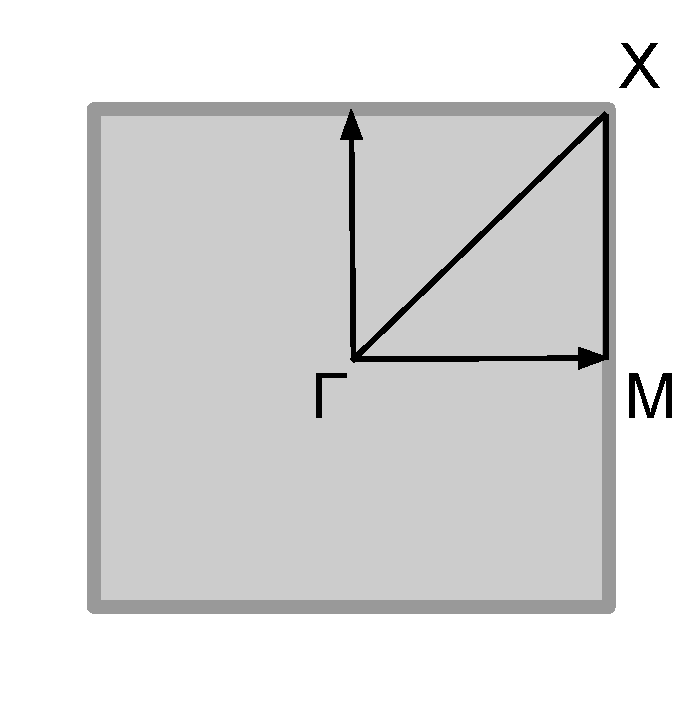
\includegraphics[width=0.25\textwidth]{twodunifcell.pdf}
	\caption{Unit cell for the homogeneous material}
	\label{fig:twodunifcell}
\end{figure}

The result of solving the eigenvalue equation along the (IBZ) is shown in 
Figure \ref{fig:twodunif}. The dispersion relation is considerably more complex 
and it appears that for a given frequency there are sometime two possible 
wavenumbers along each side of the IBZ. These degeneracies are due to the fact 
that the 2D material supports longitudinal and transverse waves. Most of the 
dispersion curves are straight which is expected for a uniform material. The 
curved lines can be attributed to Bloch harmonics \cite{veres13}.
\begin{figure}[!htbp]
	\centering
	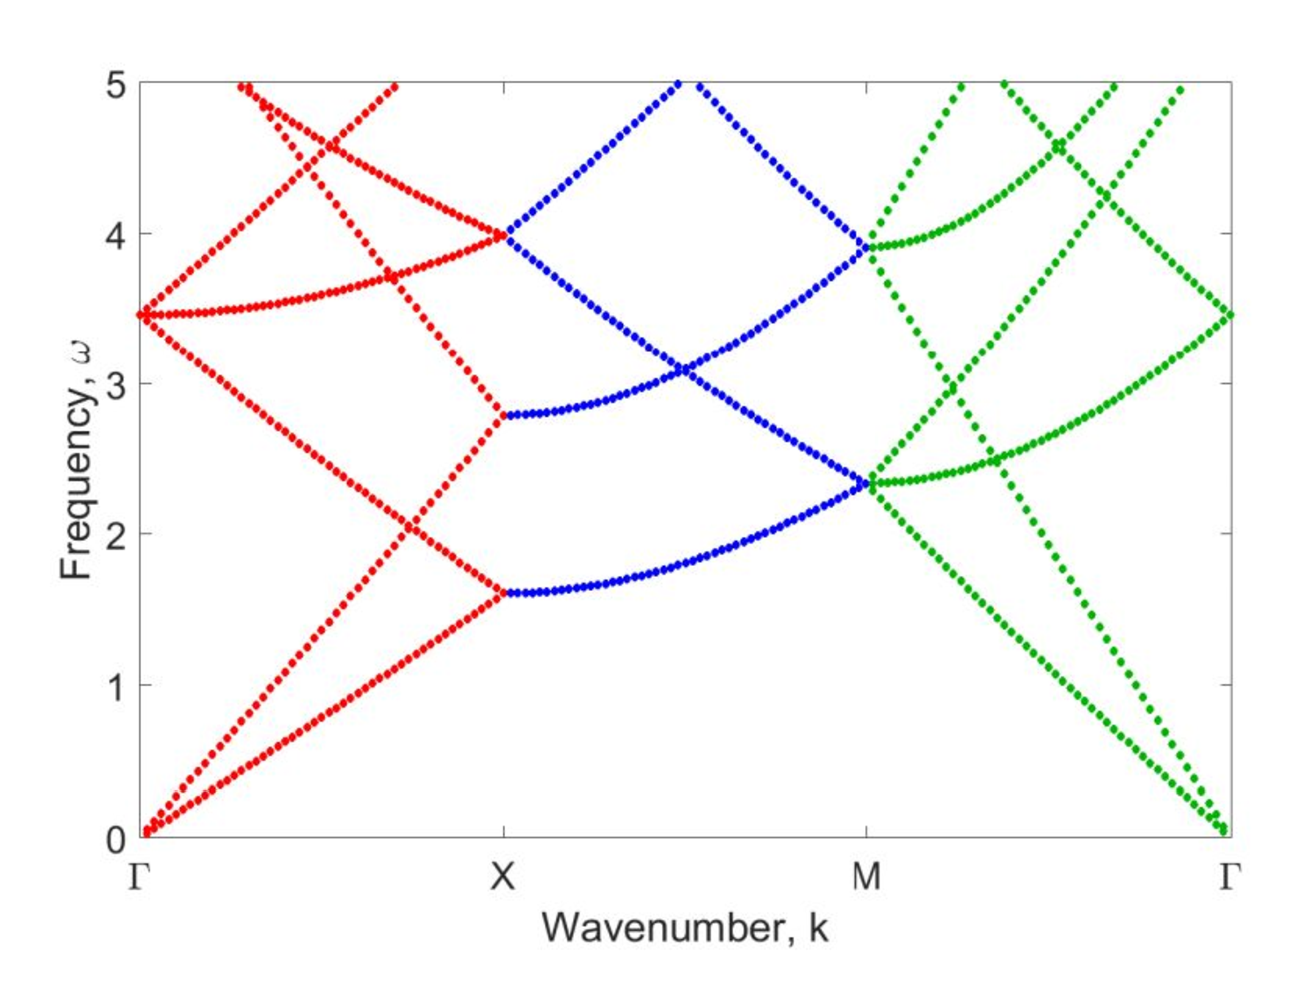
\includegraphics[width=0.8\textwidth]{twodunif.pdf}
	\caption{Dispersion relation for the 2D homogeneous material plotted along 
	the IBZ}
	\label{fig:twodunif}
\end{figure}

\subsection{Laminate}
A similar analysis is performed for a laminate with one material phase with 
$\lambda_1 = 160$, $\mu_1 = 1$, and $\rho_1 = 8$ surrounded by a second 
material phase with $\lambda_2 = \mu_2 = \rho_2 = 1$ on the outside of the unit 
cell.
\begin{figure}[!htbp]
	\centering
	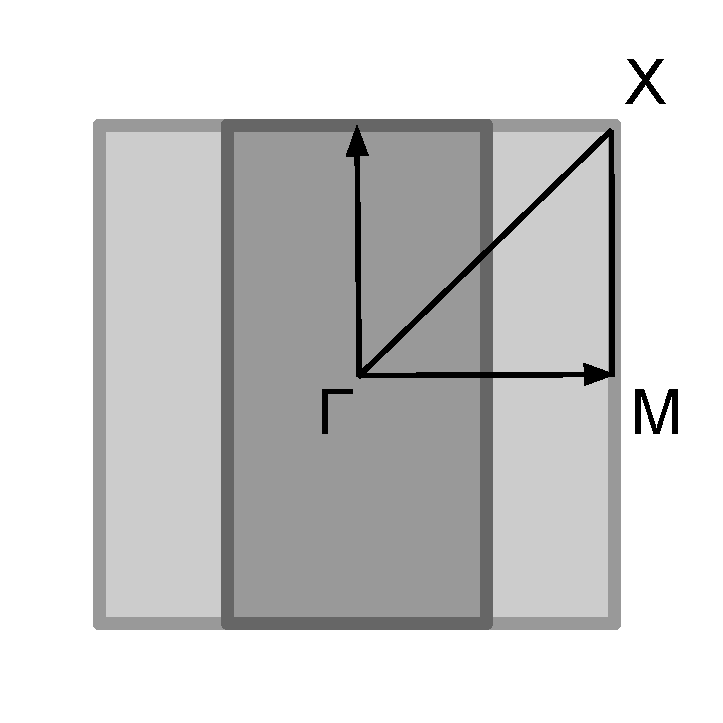
\includegraphics[width=0.25\textwidth]{twodlayrdcell.pdf}
	\caption{Unit cell for the laminate}
	\label{fig:twodlayrdcell}
\end{figure}


\begin{figure}[!htbp]
	\centering
	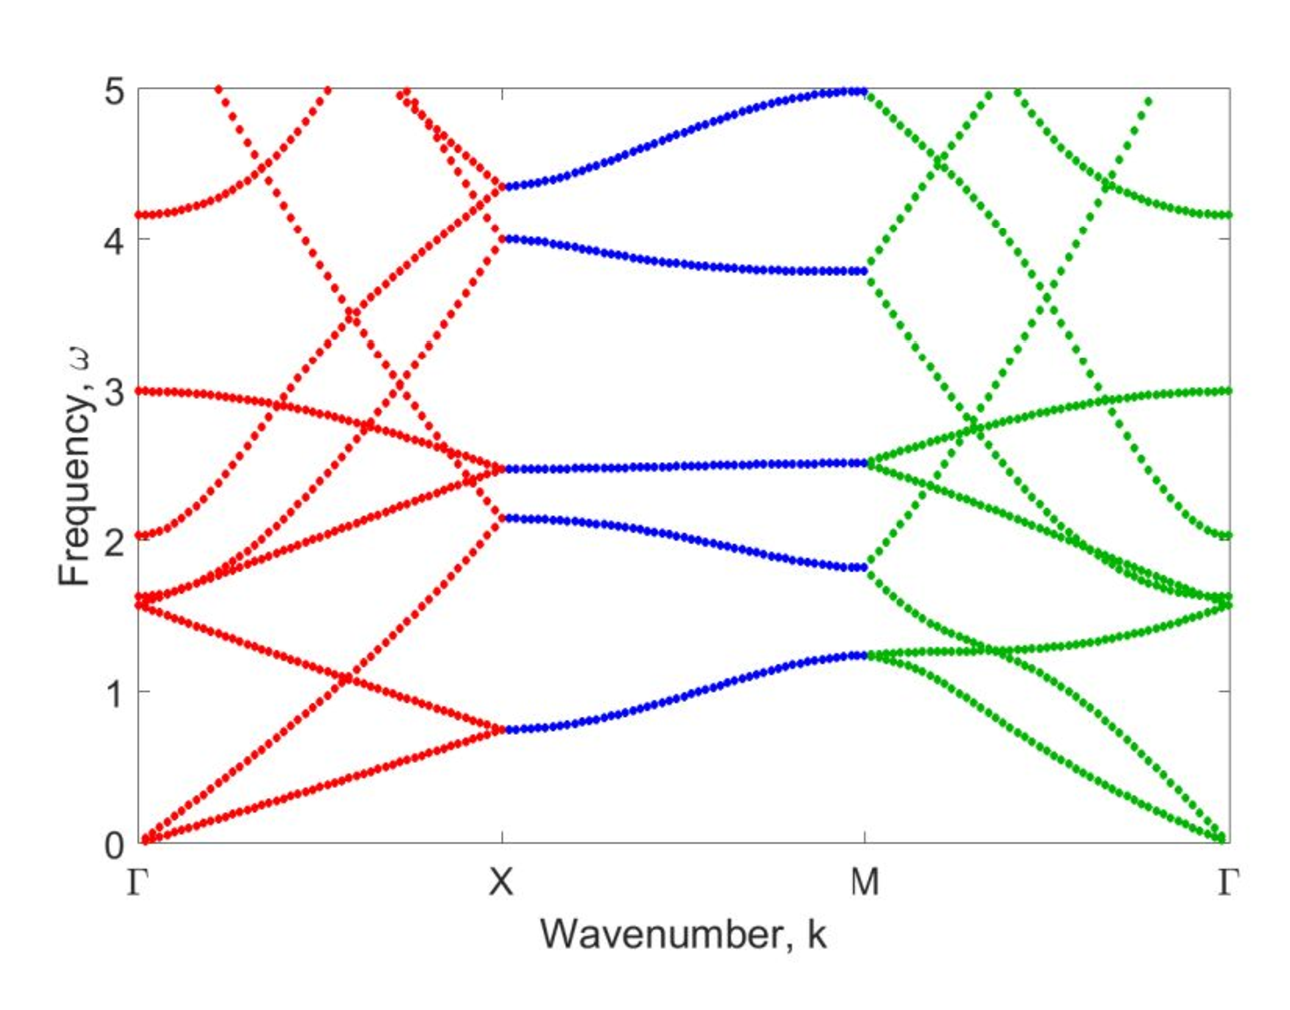
\includegraphics[width=0.8\textwidth]{twodlayrd.pdf}
	\caption{Dispersion relation for the laminate plotted along the IBZ}
	\label{fig:twodlayrd}
\end{figure}

\subsection{Material with inclusions}
\begin{figure}[!htbp]
	\centering
	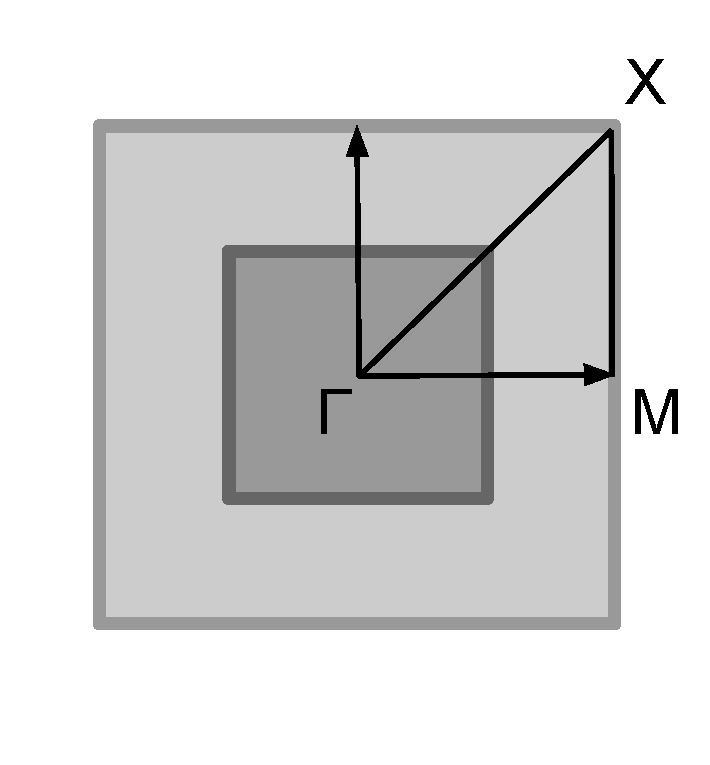
\includegraphics[width=0.25\textwidth]{twodrescell.pdf}
	\caption{Unit cell for the 2D material with square inclusions}
	\label{fig:twodrescell}
\end{figure}
\begin{figure}[!htbp]
	\centering
	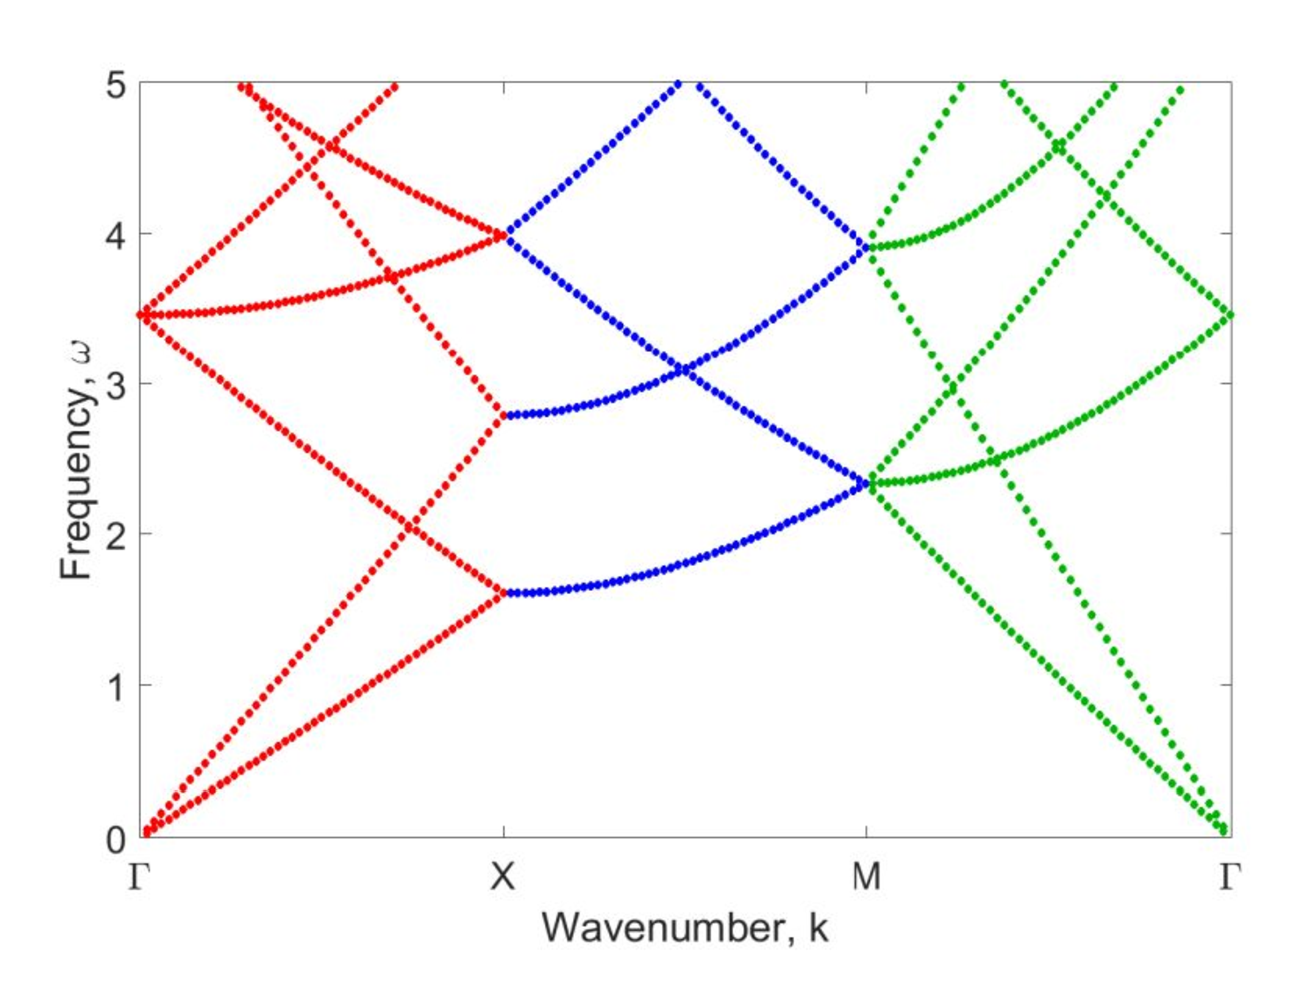
\includegraphics[width=0.8\textwidth]{twodunif.pdf}
	\caption{Dispersion relation for the 2D material with 
	square inclusions plotted along the IBZ}
	\label{fig:twodres}
\end{figure}

%------------------------------- FUTURE WORK  ---------------------------------%
%  This one will be a little difficult. Assuming you have done your literature 
%  review correctly, you should be in a position to speak about the direction 
%  you will take. This is where you take ownership of this project. Be sure to 
%  Connect with the methods of analysis you have been talking about here, but
%  also to the beginning of this report where you have outlines the frontiers
%  of research in phononic media.
%------------------------------------------------------------------------------%
\section{Future work}
In the near future it would be interesting to examine the effect of disorder on 
the diatomic mass spring system. Additionally, it would be of interest to 
develop a finite element method for analysis of disordered materials. Perhaps a 
modification of the Bloch condition or the consideration of ``supercell" may be 
what is needed.

Additionally, it is of future research interest to explore dynamic 
homogenization of these phononic media. This is going to require a more 
thorough knowledge of static homogenization theory such that a generalization 
may be made.

%-------------------------------- CONCLUSION  ---------------------------------%
%  Recapitulate and make sure that the audience knows that you are in a 
%  position to make contributions to the field. This part is important. Once 
%  again frame it so they know what has been done in the field and what hasn't.
%  The things you need to do what hasn't been done and how you have mastered 
%  them.
%------------------------------------------------------------------------------%
\section{Conclusion}
At the heart of research in phononic media, dispersion relations encapsulate a 
majority of the information needed to characterize the wave propagation in 
materials. In this independent study, a large amount of effort was put into 
developing the analytical and computational skills needed to calculate 
dispersion relations. As such, we are well poised to thrust ourselves into one 
of the active research areas of damping, nonlinear systems, or disordered 
systems and soon enough should be able to study dynamic homogenization of these 
phononic media. 

%------------- ADDITIONAL STUDIES OF HETEROGENEOUS MATERIALS  -----------------%
%  Here quickly outline the chapters of the lecture notes that you studied and 
%  some of the techniques that you have learned. Much like the proposal for 
%  this independent study
%------------------------------------------------------------------------------%
\section{Additional studies of heterogeneous materials}
In addition to this study of phononic media, much time and effort was put into 
the notes of Prof. Ponte-Casta\~neda. Attached to this document, are solutions 
to various problems in the lecture notes. 

\section{Acknowledgements}
I would like to thank my advisors Prof. Ponte-Casta\~neda and Prof. Reina for
guidance this semester. Additionally, I would like to thank Chenchen Liu of
Prof. Reina's group for helping me get a grip of using finite elements and Bloch
analysis for this phononic media.

\appendix
\section{Appendix}
\subsection{Verlet integration} \label{verlet}
For a single particle, the Verlet integration method is used to calculate its 
trajectory given that the forces (and therefore the acceleration) are known. 
The algorithm is
\begin{equation}
x^{t+1}_{n} = 2x^{t}_{n} - x^{t-1}_{n} + a(x^{t}_n)\Delta t^2
\end{equation}
where $t$ denotes the current time step, $x$ is the particle position, $a(x_n)$ 
is the acceleration, and $\Delta t$ is suitably small time step. b

\subsection{Finite difference in time for real time evolution FEM} 
\label{femrte}
For equation (\ref{matrixform}), it is possible to apply a finite difference 
method in time in order to get the real time evolution of the uniform bar. 
First, in order to apply the displacement boundary conditions at the left 
boundary, we need to modify (\ref{matrixform}). We partition the matrices 
\begin{equation} \label{partition}
\begin{bmatrix}
K_{11} & K_{1a} \\
K_{a1} & K_{aa}
\end{bmatrix}
\begin{bmatrix}
a_1 \\
a
\end{bmatrix}
+
\begin{bmatrix}
M_{11} & M_{1a} \\
M_{a1} & M_{aa}
\end{bmatrix}
\begin{bmatrix}
\ddot{a_1} \\
\ddot{a}
\end{bmatrix}
= 0
\end{equation}
Here, $K_{11}$ and $M_{11}$ denote the entry in the first row and first column. 
$K_{1a}$ and $M_{1a}$ are row vectors of the rest of the entries in the first 
row and $K_{a1}$ and $M_{a1}$ are column vectors of the remaining elements of 
the first column. $K_{aa}$ and $M_{aa}$ are then matrices of the remaining 
elements of the matrices $K$ and $M$. Since we know $a_1$ and $\ddot{a_1}$ 
(these are the displacement and acceleration at the first node), we only wish 
to solve the bottom row of ($\ref{partition}$).
\begin{equation}
K_{aa}a + M_{aa}\ddot{a} = -a_1K_{a1} - \ddot{a_1}M_{a1}
\end{equation}

To solve the above we discretize $\ddot{a}$ in time using an explicit finite 
difference scheme.
\begin{equation}
K_{aa}a^t + M_{aa}\frac{a^{t+1} - 2a^t + a^{t-1}}{\Delta t^2 } = 
-a_1^{t+1}K_{a1} - \ddot{a_1}^{t+1}M_{a1}
\end{equation}
Solving for $a^{t+1}$
\begin{equation}
a^{t+1} = M_{aa}^{-1}(-a_1^{t+1}K_{a1} - \ddot{a_1}^{t+1}M_{a1} - 
K_{aa}a^t)\Delta t^2 
+ 2a^t - a^{t-1}
\end{equation}

\bibliography{mybib}{}
\bibliographystyle{unsrt}

\end{document}
